\documentclass[9pt]{article}
\author{Name}
\title{Labs EmbSW2}
\usepackage[left=5mm,right=5mm,top=5mm,bottom=15mm]{geometry}
\usepackage{slashed}
\usepackage{graphicx}
\usepackage{pdfpages}
\usepackage{listings}
\usepackage{amsmath}
\usepackage{enumitem}
\usepackage{xcolor}
\usepackage{stackengine}
\usepackage{url}
\usepackage{multicol}
\usepackage{color} %red, green, blue, yellow, cyan, magenta, black, white
\definecolor{mygreen}{RGB}{28,172,0} % color values Red, Green, Blue
\definecolor{mylilas}{RGB}{170,55,241}
\definecolor{backcolour}{rgb}{0.95,0.95,0.95}
\lstdefinestyle{C++}{
numbers=left,
  belowcaptionskip=1\baselineskip,
  breaklines=true,
  breakatwhitespace=false,
  frame=l,
  framerule=0pt,
  postbreak=\mbox{\textcolor{red}{$\hookrightarrow$}\space},
  framesep=-1pt,
  xleftmargin=1em,
  language=C++,
  showstringspaces=false,
  basicstyle=\scriptsize\ttfamily,
  keywordstyle=\bfseries\color{green!40!black},
  commentstyle=\itshape\color{purple!40!black},
  identifierstyle=\color{blue},
  stringstyle=\color{red},
  numberstyle=\ttfamily\tiny,
  backgroundcolor=\color{backcolour}
}

\setitemize{noitemsep,topsep=0pt,parsep=0pt,partopsep=0pt}
\setlength\parindent{0pt}

\begin{document}



\maketitle
\setcounter{tocdepth}{2}
\tableofcontents

\section{Lab 1 Listen}
%!TEX root = ../prak.tex
\section{Lab 1 Listen}
\subsection{Aufgabe 1: Realisierung einer einfach verketteten Liste}
Implementieren Sie eine einfach verkettete Liste für double-Werte in C++ mit der Entwicklungsumgebung
Eclipse. Die Listenklasse erhält den Namen SList.
SList soll die nachfolgenden Methoden anbieten, wobei die geeigneten Parameter noch zu definieren sind.
Achten Sie auf den korrekten Einsatz von const.
\begin{itemize}
\item Nehmen Sie als Ausgangspunkt das vorgegebene Eclipse-Projekt. Ergänzen Sie bei Bedarf auch das einfache
Testprogramm.
\item Konstruktor (Ctor) Initialisiert eine leere Liste.
\item Destruktor (Dtor) Löscht die gesamte Liste und gibt den allozierten Speicher wieder frei.
\item \texttt{insertAt} Fügt ein Element an (nach) der bezeichneten Position ein. Einfügen am Anfang der Liste kann mittels Position 0 bewerkstelligt werden.
\item\texttt{deleteAt}
Löscht das Element an der bezeichneten Position.
\item\texttt{search}
Sucht das erste Element in der Liste mit dem definierten Wert und gibt die Position zurück. Falls das Element
nicht in der Liste vorhanden ist, wird als Position der Wert 0 zurückgegeben.
\item\texttt{isEmpty}
Gibt true zurück, falls die Liste leer ist.
\item\texttt{getNumber}
Gibt die Anzahl der Elemente der Liste zurück.
\item\texttt{getValue}
Gibt den Wert des Elementes an der bezeichneten Position zurück.
\item\texttt{setValue}
Setzt den Wert des Elementes an der bezeichneten Position.
\item\texttt{print}
Schreibt den Inhalt der Liste in die Console.
\end{itemize}

\subsubsection{Lösung}

\lstinputlisting[language=C++, style=C++, multicols=2]{900-Praktika/prak01/Loesung/Lists/src/SList.h}
\noindent\makebox[\linewidth]{\rule{\paperwidth}{0.4pt}}
\lstinputlisting[language=C++, style=C++, multicols=2]{900-Praktika/prak01/Loesung/Lists/src/SList.cpp}

\subsection{Aufgabe 2: Liste für beliebige Typen}

Erweitern Sie die Klasse SList so, dass beliebige Typen abgespeichert werden können. Achten Sie dabei
auch auf die korrekte Verwendung von Referenzen und des \texttt{const} Qualifiers.

Zur Erinnerung: Sie müssen hier Templates verwenden.

\subsubsection{Lösung}

\lstinputlisting[language=C++, style=C++, multicols=2]{900-Praktika/prak01/Loesung/A2/src/SList.h}

\subsection{Aufgabe 3: Realisierung einer doppelt verketteten Liste}

Implementieren Sie die Klasse \texttt{DList}, welche eine doppelt verkettete Liste für double-Werte in C++ definiert.
\texttt{DList} soll dieselben Methoden anbieten wie bereits \texttt{SList} in Aufgabe 1.
Bemerkung: hier müssen Sie keine Templates verwenden.

\subsubsection{Lösung}

\lstinputlisting[language=C++, style=C++, multicols=2]{900-Praktika/prak01/Loesung/Lists/src/DList.h}
\noindent\makebox[\linewidth]{\rule{\paperwidth}{0.4pt}}
\lstinputlisting[language=C++, style=C++, multicols=2]{900-Praktika/prak01/Loesung/Lists/src/DList.cpp}

\subsection{Aufgabe 4: Gemeinsame Basisklasse}

Die beiden Listen \texttt{SList} und \texttt{DList} haben verschiedene Gemeinsamkeiten, eine gemeinsame Basisklasse
List bietet sich offensichtlich an. Implementieren Sie eine gemeinsame Basisklasse \texttt{List}. Achten Sie darauf,
dass die Sichtbarkeiten (\texttt{public}, \texttt{private}, \texttt{protected}) so gewählt werden, dass die Unterklassen Zugriff
auf die von ihnen benötigten Daten haben. Es ist jedoch keine Lösung, einfach alles als \texttt{public} zu deklarieren.

\subsubsection{Lösung}

\lstinputlisting[language=C++, style=C++, multicols=2]{900-Praktika/prak01/Loesung/A4/src/List.h}
\noindent\makebox[\linewidth]{\rule{\paperwidth}{0.4pt}}
\lstinputlisting[language=C++, style=C++, multicols=2]{900-Praktika/prak01/Loesung/A4/src/SList.h}
\noindent\makebox[\linewidth]{\rule{\paperwidth}{0.4pt}}
\lstinputlisting[language=C++, style=C++, multicols=2]{900-Praktika/prak01/Loesung/A4/src/SList.cpp}
\noindent\makebox[\linewidth]{\rule{\paperwidth}{0.4pt}}
\lstinputlisting[language=C++, style=C++, multicols=2]{900-Praktika/prak01/Loesung/A4/src/DList.h}
\noindent\makebox[\linewidth]{\rule{\paperwidth}{0.4pt}}
\lstinputlisting[language=C++, style=C++, multicols=2]{900-Praktika/prak01/Loesung/A4/src/DList.cpp}

\subsection{Aufgabe 5: Gemeinsame Basisklasse mit Templates}

Die komfortabelste Lösung ist offensichtlich, die beiden Klassen \texttt{SList} und \texttt{DList} als Templateklassen zu implementieren mit einer gemeinsamen Basisklasse.

\subsubsection{Lösung}

\lstinputlisting[language=C++, style=C++, multicols=2]{900-Praktika/prak01/Loesung/A5/src/List.h}
\noindent\makebox[\linewidth]{\rule{\paperwidth}{0.4pt}}
\lstinputlisting[language=C++, style=C++, multicols=2]{900-Praktika/prak01/Loesung/A5/src/SList.h}
\noindent\makebox[\linewidth]{\rule{\paperwidth}{0.4pt}}
\lstinputlisting[language=C++, style=C++, multicols=2]{900-Praktika/prak01/Loesung/A5/src/DList.h}
\noindent\makebox[\linewidth]{\rule{\paperwidth}{0.4pt}}
\lstinputlisting[language=C++, style=C++, multicols=2]{900-Praktika/prak01/Loesung/A5/src/ListTest.cpp}

\newpage
\section{Lab 2 Listen, Algorithmen und Komplexitätstheorie}
\subsection{Aufgabe 1: Klasse für die Speicherung von Messwerten}
Als Vorgabe erhalten Sie eine Templateklasse für eine einfach verkettete Liste. Implementieren Sie darauf basierend eine Klasse für die Verwaltung von Messreihen. Die Klasse speichert eine beliebige Anzahl von Messwerten. Einer zu implementierenden Methode können Sie einen Toleranzwert in Prozent übergeben. Die Methode entfernt dann aus der Liste alle Messwerte, die mehr als dieser Toleranzwert vom Mittelwert der Messwerte abweichen.
Überlegen Sie sich als erstes, ob die Beziehung zur Listenklasse eine Vererbung oder eine Aggregation ist. Begründen Sie Ihre Wahl.

\subsubsection{Lösung}
Die Messwertliste ist eine Liste, deshalb ist aus objektorientierter Sicht eine Vererbungsbeziehung vorzuziehen.

\large{Vererbung:}
\lstinputlisting[language=C++, style=C++, multicols=2]{900-Praktika/prak02/Loesung/MeasureListInh/src/MeasureList.h}
\noindent\makebox[\linewidth]{\rule{\paperwidth}{0.4pt}}
\lstinputlisting[language=C++, style=C++, multicols=2]{900-Praktika/prak02/Loesung/MeasureListInh/src/MeasureList.cpp}
\noindent\makebox[\linewidth]{\rule{\paperwidth}{0.4pt}}
\lstinputlisting[language=C++, style=C++, multicols=2]{900-Praktika/prak02/Loesung/MeasureListInh/src/SList.h}
\noindent\makebox[\linewidth]{\rule{\paperwidth}{0.4pt}}
\lstinputlisting[language=C++, style=C++, multicols=2]{900-Praktika/prak02/Loesung/MeasureListInh/src/MListMain.cpp}

\large{Aggregation}
\lstinputlisting[language=C++, style=C++, multicols=2]{900-Praktika/prak02/Loesung/MeasureListAgg/src/MeasureList.h}
\noindent\makebox[\linewidth]{\rule{\paperwidth}{0.4pt}}
\lstinputlisting[language=C++, style=C++, multicols=2]{900-Praktika/prak02/Loesung/MeasureListAgg/src/MeasureList.cpp}
\noindent\makebox[\linewidth]{\rule{\paperwidth}{0.4pt}}
\lstinputlisting[language=C++, style=C++, multicols=2]{900-Praktika/prak02/Loesung/MeasureListAgg/src/SList.h}
\noindent\makebox[\linewidth]{\rule{\paperwidth}{0.4pt}}
\lstinputlisting[language=C++, style=C++, multicols=2]{900-Praktika/prak02/Loesung/MeasureListAgg/src/MListMain.cpp}

\subsection{Aufgabe 2: Komplexitätsbetrachtungen}
Bestimmen Sie den benötigten Aufwand der folgenden Algorithmen in $O$-Notation. Alle Algorithmen berech-nen die Potenz $c=a^b$.
\begin{lstlisting}[language=C++, style=C++, multicols=2]
/ berechnet 'a^^b', Voraussetzung: b>=0
double potenz1(double a, int b)
{
    double c = 1;
    while (b > 0)
    {
        c = c * a;
        b = b - 1;
    }
    return c;
    }
        // berechnet 'a^^b', Voraussetzung: b>=0
        double potenz2(double a, int b)
        {
        if (b == 0)
        return 1;
        else
        return potenz2(a, b-1) * a;
    }
    // berechnet 'a^^b', Voraussetzung: b>=0
    double potenz3(double a, int b)
    {
        double c = 1;
        while (b > 0)
    {
        if (b % 2 == 1)
        c = c * a;
        a = a * a;
        b = b / 2;
    }
    reeturn c;
}
\end{lstlisting}
\subsubsection{Lösung}
In der Funktion \texttt{potenz1()} wird die \texttt{while}-Schleife b mal durchlaufen, d.h. dieser Algorithmus ist $O(b)$.
Die Funktion \texttt{potenz2()} wird b mal rekursiv aufgerufen, weitere Schleifen sind nicht vorhanden, d.h. dieser Algorithmus ist $O(b)$.
In der Funktion \texttt{potenz3()} wird b bei jedem Schleifendurchlauf halbiert. Die Schleife wird ungefähr $ld(b$) mal durchlaufen (ld = logarithmus dualis, Zweierlogarithmus). \texttt{potenz3()} ist demnach $O(log b)$.

\subsection{Aufgabe 3: Implementation eines dynamischen Stacks mit Hilfe einer verketteten Liste}
Ein Stack (Stapel, LIFO, Last-In-First-Out) ist eine Datenstruktur, bei der das Element, das zuerst auf den Stack gespeichert wird, als letztes wieder ausgelesen wird.

Implementieren Sie eine Klasse \texttt{Stack}, die nicht auf Arrays, sondern mit der vorgegebenen einfach verket-teten Liste arbeitet. Die \texttt{Stack}-Klasse soll als Template implementiert sein.
Überlegen Sie sich auch hier als erstes, ob die Beziehung zur Listenklasse eine Vererbung oder eine Aggre-gation ist. Begründen Sie Ihre Wahl.

Als Methoden müssen Sie die bekannten Stackoperationen \texttt{push()}, \texttt{pop()}, \texttt{isEmpty()} und \texttt{peek()} realisie-ren. Reservieren Sie im Konstruktor die als Parameter übergebene Anzahl Listenelemente. Falls ein push() bei einem vollen Stack probiert wird, soll jetzt aber nicht ein Fehler ausgegeben werden, stattdessen sollen Sie den Stack dynamisch um zusätzliche Elemente vergrössern.

\subsubsection{Lösung}
Der Stack ist nicht eine Liste, er benutzt nur eine für die Speicherung der Daten. Eine Vererbung kommt deshalb nicht in Frage, Aggregation ist die richtige Variante. Da der Stack beliebige Daten speichern können soll, muss er unbedingt als Templateklasse implementiert werden.

\lstinputlisting[language=C++, style=C++, multicols=2]{900-Praktika/prak02/Loesung/DynaStack/SList.h}
\noindent\makebox[\linewidth]{\rule{\paperwidth}{0.4pt}}
\lstinputlisting[language=C++, style=C++, multicols=2]{900-Praktika/prak02/Loesung/DynaStack/Stack.h}
\noindent\makebox[\linewidth]{\rule{\paperwidth}{0.4pt}}
\lstinputlisting[language=C++, style=C++, multicols=2]{900-Praktika/prak02/Loesung/DynaStack/stacktest.cpp}
\noindent\makebox[\linewidth]{\rule{\paperwidth}{0.4pt}}
\lstinputlisting[language=C++, style=C++, multicols=2]{900-Praktika/prak02/Loesung/DynaStack/StackUI.h}

\newpage
\section{Lab 3 Sortieralgorithmen und Komplexitätstheorie}
\subsection{Aufgabe 1: Zeitmessung bei Fibonacci-Implementationen}
Sie erhalten als Vorgabe die beiden Dateien fiboit.c und fiborek.c. Sie beinhalten eine iterative Implementation
der Fibonacci-Zahlen, respektive eine rekursive Implementation, jeweils in der Programmiersprache
C.
\begin{enumerate}
  \item Implementieren Sie die beiden Programme je in C++ (sie müssen nicht objektorientiert sein).
  \item Sie haben gesehen, dass die rekursive Implementation mit der Fakultät wächst. Verifizieren Sie die Theorie, indem Sie Zeitmessungen für die Berechnung vornehmen.
\end{enumerate}

\textbf{Hinweis zu den Zeitmessungen:}

Mit einfachen Mitteln ist eine genaue absolute Zeitmessung nicht durchführbar. Für unsere Zwecke genügt
hier eine relative Zeitmessung, die genügend genau ist. Wählen Sie eine der folgenden Varianten:

Variante 1: Messung der Standardzeit

Die Funktion \texttt{clock()} aus \texttt{<ctime>} liefert die abgelaufene CPU-Zeit in Clockticks seit Programmstart. Wenn
diese Grösse durch \texttt{CLOCKS\_PER\_SEC} geteilt wird, erhält man eine Zeit in Sekunden.
\begin{lstlisting}[language=C++, style=C++]
#include <ctime>
clock_t start = clock();
// do something
clock_t end = clock();
cout << "Ticks: " << end-start << endl;
cout << "Time: " << static_cast<double>(end-start) / CLOCKS_PER_SEC << " sec" << endl;
\end{lstlisting}

Variante 2: Native Zeitmessung von Linux
\begin{lstlisting}[language=C++, style=C++]
#include <sys/resource.h>
#include <sys/types.h>
rusage tp;
double start; // Startzeit in Millisekunden
double end; // Endzeit
getrusage(RUSAGE_SELF, &tp);
start = static_cast<double>(tp.ru_utime.tv_sec) +
        static_cast<double>(tp.ru_utime.tv_usec)/1E6;
// do something
getrusage(RUSAGE_SELF, &tp);
end = static_cast<double>(tp.ru_utime.tv_sec) +
      static_cast<double>(tp.ru_utime.tv_usec)/1E6;
cout << "Dauer: " << end-start << " sec" << endl;
\end{lstlisting}

\subsubsection{Lösung}

\large{Iterativ + Linux Zeitmessung}
\lstinputlisting[language=C++, style=C++, multicols=2]{900-Praktika/prak03/Loesung/FiboItWatch/fiboit.cpp}

\large{Rekursiv + \texttt{clock()} Zeitmessung}
\lstinputlisting[language=C++, style=C++, multicols=2]{900-Praktika/prak03/Loesung/FiboRekWatch/fiborek.cpp}

\large{Rekursiv + Linux Zeitmessung}
\lstinputlisting[language=C++, style=C++, multicols=2]{900-Praktika/prak03/Loesung/FiboRekWatchLinux/fiborek.cpp}

\subsection{Aufgabe 2: Klasse für Stoppuhr}
Implementieren Sie eine Klasse \texttt{StopWatch}, die sich bei der Gründung eines Objekts die Zeit merkt. Bei
jedem Aufruf der Methode \texttt{elapsed()} wird die bis dahin abgelaufene Zeit in Sekunden zurückgegeben.
Beispiel:

\begin{lstlisting}[language=C++, style=C++]
StopWatch t; // starts stopwatch
double d = t.elapsed();
\end{lstlisting}

\subsubsection{Lösung}

\lstinputlisting[language=C++, style=C++, multicols=2]{900-Praktika/prak03/Loesung/StopWatch/src/StopWatch.h}
\noindent\makebox[\linewidth]{\rule{\paperwidth}{0.4pt}}
\lstinputlisting[language=C++, style=C++, multicols=2]{900-Praktika/prak03/Loesung/StopWatch/src/StopWatch.cpp}
\noindent\makebox[\linewidth]{\rule{\paperwidth}{0.4pt}}
\lstinputlisting[language=C++, style=C++, multicols=2]{900-Praktika/prak03/Loesung/StopWatch/src/StopWatchTest.cpp}

\subsection{Aufgabe 3: Komplexität}

Es gilt die Annahme, dass ein gewisses Programm jeden Abend exakt eine Stunde Rechenzeit bekommt.
Sie haben herausgefunden, dass das Programm $n=1'000'000$ Datensätze verarbeiten kann. Nun wird ein
neuer Rechner angeschafft, der 100 Mal schneller als der alte ist.
Wie viele Datensätze kann Ihr Programm nun in einer Stunde verarbeiten, wenn wir die folgende Zeitkomplexität
mit den Konstanten $k_i$ annehmen?

\begin{enumerate}
  \item $k_1 \cdot n$
  \item $k_2 \cdot n \cdot \log_{10} n$
  \item $k_3 \cdot n^2$
  \item $k_4 \cdot n^3$
  \item $k_5 \cdot 10^n$
\end{enumerate}

\textbf{Hinweis:}
Verwenden Sie den Ansatz, dass der schnelle Rechner in einer Stunde gleich viel leistet, wie der
langsame in 100 Stunden.

\subsubsection{Lösung}

\textbf{Ansatz:}

\begin{itemize}
  \item Langsamer Rechner: $T(n) = 1 \text{h}$
  \item Schnellerer Rechner : 100 Mal Schneller
  \begin{itemize}
    \item Der schnellere Rechner leistet in 1h gleich viel wie der langsamere in 100 h.
    \begin{enumerate}
      \item $T(n) = 1$ für $n= 10^6$ einsetzen $\Rightarrow$ ergibt $k$;
      \item $T(n)\mathrel{\stackon[1pt]{$=$}{$\scriptstyle!$}} 100 $ setzen mit unter (1.) ermitteltem $k$;
      \item nach $n$ auflösen
        \end{enumerate}
  \end{itemize}
\end{itemize}

\noindent
\textbf{a)}

\medskip

$ k_1 \cdot 10^6 = 1 \Longrightarrow k_1 = \underline{10^{-6}}$

$ k_1 \cdot n = 100 \Longrightarrow n = \frac{1}{k} \cdot 100 = 10^6 \cdot 100 = \underline{\underline{10^8}}$

\noindent
\textbf{b)}
\medskip

$ k_2 \cdot 10^6\cdot \log_{10} 10^6 = 1$

$\Rightarrow k_2 \cdot 10^6 \cdot 6 = 1 \Rightarrow k_2 = \frac{1}{6} \cdot \underline{10^-6}$

$ \Rightarrow k_2 \cdot n \cdot \log_{10} n = 100$

$ \Rightarrow n \cdot \log_{10} n = 6 \cdot 10^8 =: c_2 $

$\Rightarrow 10^{n \cdot \log_{10} n} = 10^{c_2}$

$\Rightarrow n^n = 10^{c_2} = 10^{6\cdot10^8}$

Diese Gleichung lasst sich nicht geschlossen lösen.

solver: $\underline{\underline{n= 76 127 253}}$

\noindent
\textbf{c)}
\medskip

$ k_3 \cdot (10^6)^2 = 1 $

$\Rightarrow k_3 \cdot 10^12 = 1 \Rightarrow k_3 = \underline{10^{-12}}$

$k_3 \cdot n^2 = 100$

$\Rightarrow \underline{n} = \sqrt{10^{14}} = \underline{\underline{10^7}}$

\noindent
\textbf{d)}
\medskip

$ k_4\cdot (10^6)^3 = 1$

$\Rightarrow k_4 \cdot 10^{18} =1 \Rightarrow k_4 = \underline{10^{-18}}$

$k_4 \cdot n^3 = 100 \Rightarrow n^3 = 10^{20}$

$\Rightarrow \underline{n} = 10^{\frac{20}{3}} = \underline{\underline{4641588}}$

\noindent
\textbf{e)}
\medskip

$ k_5 \cdot 10^{10^6} = 1 \Rightarrow k_5 = \underline{\frac{1}{10^{10^6}}}$

$ k_5 \cdot 10^{n} = 100$

$ \Rightarrow 10^n = 100 \cdot  10^{10^6} =  10^{10^6+2}$

$\Rightarrow \underline{n} = 10^{6} + 2 = \underline{\underline{1000002}}$

d.h. mit einem 100 Mal schnelleren Rechner können Sie 2 (!) zusätzliche Datensätze berechnen.

\subsection{Aufgabe 4: Sortieralgorithmen}
Implementieren Sie einen rekursiven Quicksort-Algorithmus, der für Teildaten mit weniger als $M$ Elementen
zu Insertionsort (Direktes Einfügen) übergeht.

Bestimmen Sie empirisch den optimalen Wert von $M$. Nehmen Sie einen Array mit ungefähr fünf Millionen
zufällig erzeugten Ganzzahlen an und messen Sie, mit welchem $M$ die Sortierung am schnellsten abgearbeitet
wird. Betrachten Sie dabei sowohl das Sortieren der unsortierten als auch der bereits sortierten Liste.



\subsubsection{Lösung}

Mit dem verwendeten Rechner wurde die Listengrösse mit 5 Mio. Elementen des Typs int gewählt. Die Lis-te musste auf dem Heap angelegt werden, beim Einsatz einer Stackvariablen resultierte ein Stackoverflow.

In Abbildung 1 sind die Laufzeitmessungen dargestellt (Execution time in Sekunden). Wenn die Schwelle auf Null gesetzt wird, gibt es keinen Wechsel des Algorithmus, d.h. das ist der reine Quicksort-Algorithmus. Aus den Messungen ist ersichtlich, dass das Sortieren der unsortierten Liste am schnellsten ist, wenn unterhalb einer Listengrösse von ca. 30-80 auf den Insertionsort umgestellt wird (obere Kurve 'Unsorted'). Wenn die Liste bereits sortiert ist, dann schneidet der reine Quicksort nicht schlechter ab (mittlere Kurve 'Sorted'). Auf-grund der Kombination dieser beider Kurven ist es sinnvoll, die Schwelle auf ca. 30 zu setzen.
Die unterste Kurve stellt das Messrauschen, d.h. die Abweichung bei mehreren Messungen, dar bei der Sortierung von unsortierten Listen. Das Messrauschen ist doch recht hoch.

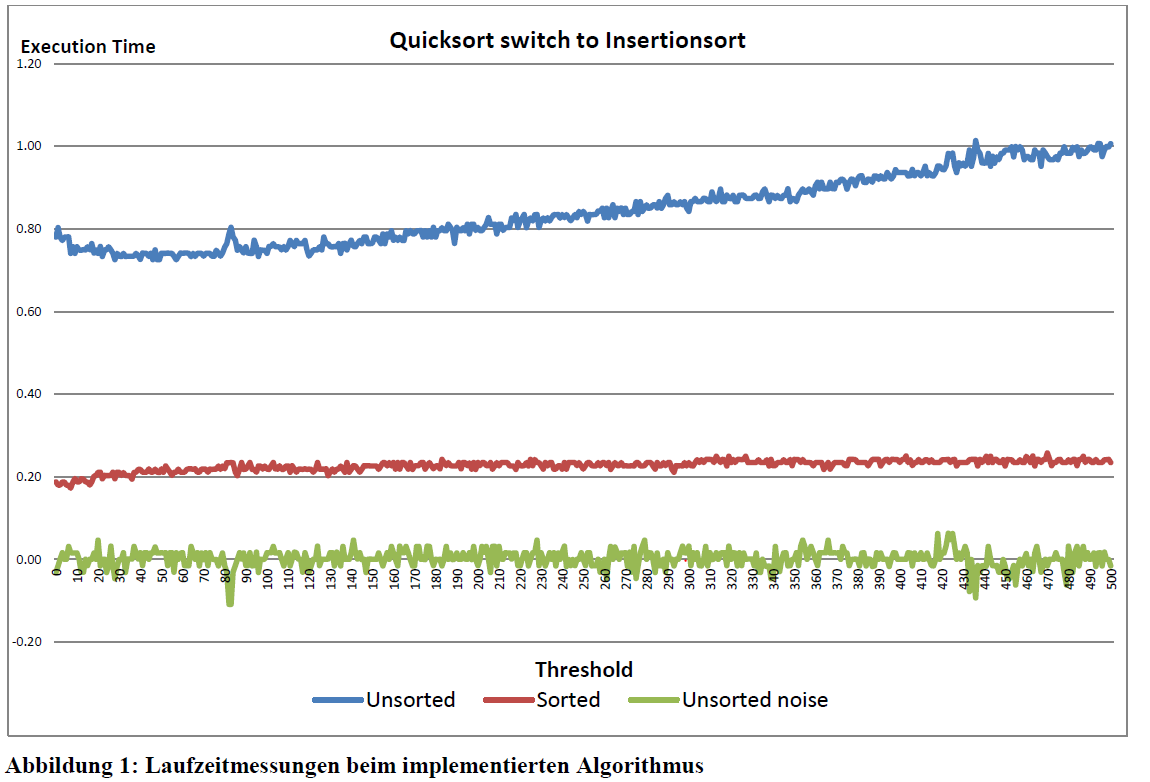
\includegraphics[width=.8\linewidth]{900-Praktika/prak03/pic.PNG}


\lstinputlisting[language=C++, style=C++, multicols=2]{900-Praktika/prak03/Loesung/QuickSortFast/src/List.h}
\noindent\makebox[\linewidth]{\rule{\paperwidth}{0.4pt}}
\lstinputlisting[language=C++, style=C++, multicols=2]{900-Praktika/prak03/Loesung/QuickSortFast/src/List.cpp}
\noindent\makebox[\linewidth]{\rule{\paperwidth}{0.4pt}}
\lstinputlisting[language=C++, style=C++, multicols=2]{900-Praktika/prak03/Loesung/QuickSortFast/src/QuickSortFast.cpp}
\noindent\makebox[\linewidth]{\rule{\paperwidth}{0.4pt}}
\lstinputlisting[language=C++, style=C++, multicols=2]{900-Praktika/prak03/Loesung/QuickSortFast/src/StopWatch.h}
\noindent\makebox[\linewidth]{\rule{\paperwidth}{0.4pt}}
\lstinputlisting[language=C++, style=C++, multicols=2]{900-Praktika/prak03/Loesung/QuickSortFast/src/StopWatch.cpp}
\noindent\makebox[\linewidth]{\rule{\paperwidth}{0.4pt}}

\newpage
\section{Lab 4 Zufallszahlengeneratoren}
\subsection{Aufgabe 1: Verteilung der Zufallswerte durch \texttt{rand()}}

\texttt{rand()} liefert gleichverteilte Werte zwischen 0 und inklusive \texttt{RAND\_MAX}, d.h im Intervall \texttt{[0, RAND\_MAX]}. Untersuchen Sie, wie gut diese Gleichverteilung eingehalten wird. Dazu soll das Testprogramm zufällige Zahlen im Bereich von [1, 20] liefern. Speichern Sie die Anzahl in einem Array und stellen Sie das Resul-tat in einem GUI oder mit Hilfe von Excel dar.
Hinweis: die man-Page für die Funktion \texttt{rand()} erhalten Sie mit Hilfe des Befehls \texttt{man 3 rand}

\subsubsection{Lösung}

Das Eclipse-Projekt ist in ./Loesung/RandDist zu finden. Bei einer Umrechnung in einen bestimmten Be-reich ist wichtig, dass alle Werte, insbesondere auch der grösste und der kleinste, gleichverteilt sind. Die ein-fachste Umrechnung kann mit Hilfe des Modulooperators \% erreicht werden. Allerdings werden dann nur die niederwertigsten Bits der Zufallszahl berücksichtigt. Dies kann zu wenig zufälligen Folgen führen. Beachten Sie auch die Kommentare im Code.

In der folgenden Abbildung sind die Verteilungen bei 20'000, bzw. bei 2'000'000 Zufallszahlen dargestellt.
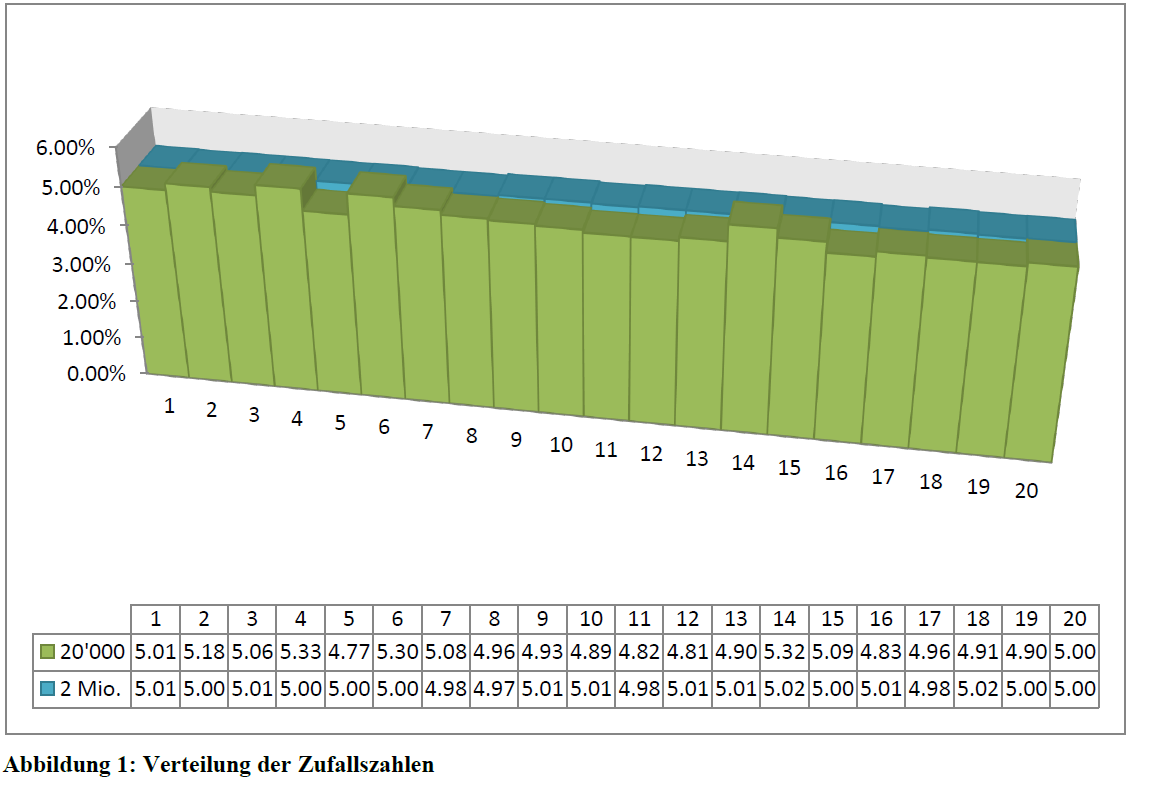
\includegraphics[width=.8\linewidth]{900-Praktika/prak04/pic.PNG}

\lstinputlisting[language=C++, style=C++, multicols=2]{900-Praktika/prak04/Loesung/RandDist/src/RandDist.cpp}


\subsection{Aufgabe 2: Güte von Zufallszahlengeneratoren}
Zufallszahlen werden oft als Zahlenreihen implementiert, die mit der folgenden Formel beschrieben werden können:

\begin{equation}
  r_{i+1} = (A \cdot r_i) \% m
\end{equation}

Die Formel besteht aus einem ganzzahligen Startwert $r_0$ und mit ganzzahligen Konstanten $a$ (Multiplikator), $c $(Inkrement) und $m$ (Modulus). Diese Konstanten sind sorgfältig zu wählen, damit die Zahlen zufällig werden. So erzeugte Zahlenfolgen haben immer eine Periode $\leq$ $m$. Bei gegebenen Konstanten und Startwert $r_0$ ist die Folge eindeutig festgelegt.


Zur Beurteilung der Güte von Zufallszahlen existieren in der Statistik verschiedene Verfahren. In dieser Auf-gabe sollen Sie mit Hilfe des Computers einen graphischen Gütetest entwickeln und damit verschiedene Zu-fallszahlen-Generatoren testen. Verwenden Sie dazu Qt. Sie finden ein Qt Creator Projekt als Vorgabe.

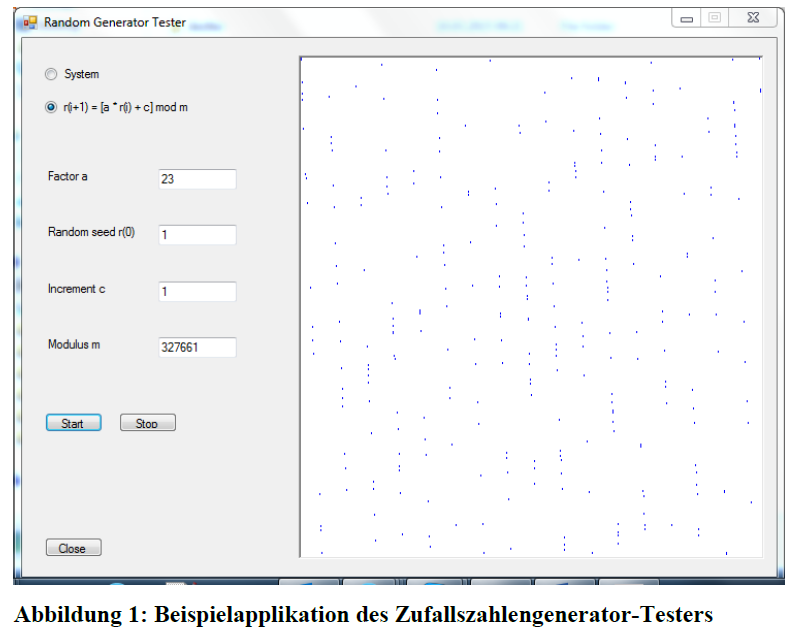
\includegraphics[width=.8\linewidth]{900-Praktika/prak04/pic2.PNG}
\begin{enumerate}
  \item Im graphischen Fenster soll ein Quadrat gezeichnet werden. Mittels zweier aufeinanderfolgender Zufalls-zahlen, die geeignet skaliert werden, wird ein Koordinatenpaar in diesem Quadrat festgelegt (1. Zufalls-zahl: x-Wert, 2. Zufallszahl: y-Wert) und an der entsprechenden Stelle ein Punkt gezeichnet. Im näch-sten Schritt wird der y-Wert zum neuen x-Wert und für den neuen y-Wert muss eine neue Zufallszahl erzeugt werden. Dieser Vorgang wird beliebig wiederholt. Durch die Beobachtung der graphischen Anordneratoren zeigen im allgemeinen ein allzu ausgeprägtes Muster. Damit das fortlaufende Zeichnen der Punkte verfolgt werden kann, wird ein Timer eingesetzt. Als Timerintervall wird 10 ms gewählt. Jedesmal wenn sich der Timer meldet, soll ein Punkt gezeichnet werden. In Ihrem Programm sollen die Werte $r_0$, $a$, $c$ und $m$ eingegeben werden können. Auf dem Skriptserver finden Sie als Muster eine vollständige ausführbare Anwendung (siehe Abbildung 1).
  \item Testen Sie z.B. die folgenden Zufallszahlengeneratoren:

  \begin{center}
           \begin{tabular}{c c c c}
           % \multicolumn{4}{ c }{\large{\textbf{Used FPGA's}}} \\
           % \multicolumn{4}{c}{} \\
           \hline
           \hline
           \textbf{$a$} &  \textbf{$r_0$} & \textbf{$c$} & \textbf{$m$} \\
           \hline

            2 & 0 & 1 & 28  \\
            8 & 0 & 1 & 7  \\
            125 & 0 & 0 & 8192  \\
            21 & 1 & 3 & 64  \\
            25 & 1 & 1 & 64  \\
            3 & 1 & 1 & 32766  \\
            130 & 1 & 1 & 32766  \\
            1331 & 1 & 1 & 327661  \\
            1103515245 & 1 & 12345 & 32768  \\

            \hline
            \hline
       \end{tabular}
   \end{center}
\item Testen Sie den Zufallszahlengenerator des Systems: rand(). Übrigens: mit Hilfe der C-Funktion srand() wird der Startwert $r_0$, der random seed, festgelegt

\end{enumerate}

\subsubsection{Lösung}

\lstinputlisting[language=C++, style=C++, multicols=2]{900-Praktika/prak04/Loesung/RandomTesterQt/main.cpp}
\noindent\makebox[\linewidth]{\rule{\paperwidth}{0.4pt}}
\lstinputlisting[language=C++, style=C++, multicols=2]{900-Praktika/prak04/Loesung/RandomTesterQt/randomtester.h}
\noindent\makebox[\linewidth]{\rule{\paperwidth}{0.4pt}}
\lstinputlisting[language=C++, style=C++, multicols=2]{900-Praktika/prak04/Loesung/RandomTesterQt/randomtester.cpp}
\noindent\makebox[\linewidth]{\rule{\paperwidth}{0.4pt}}
\lstinputlisting[language=C++, style=C++, multicols=2]{900-Praktika/prak04/Loesung/RandomTesterQt/randomviewer.h}
\noindent\makebox[\linewidth]{\rule{\paperwidth}{0.4pt}}
\lstinputlisting[language=C++, style=C++, multicols=2]{900-Praktika/prak04/Loesung/RandomTesterQt/randomviewer.cpp}

\subsection{Aufgabe 3: Nicht ideale Münze (biased coin)}
Eine ideale (faire) Münze liefert je zur Hälfte Kopf und Zahl, d.h. $p(K) = p(Z) = 0.5$. Wir nehmen nun an, die Münze sei nicht ideal, z.B.$ p(K) = 0.6, p(Z) = 0.4$.

\begin{enumerate}
  \item In ./Vorgabe/Coin/biasedCoin.cpp finden Sie die Funktion \texttt{biasedCoin()}, welche eine unfaire Mün-ze implementiert. Studieren Sie den Code und verifizieren Sie, ob die Verteilung den Erwartungen ent-spricht.
  \item Entwickeln Sie einen Algorithmus, der mit einer beliebig konstant unfairen Münze einen gleichverteilten Zufallsprozess erreichen kann. Implementieren Sie den Code, dabei müssen Sie die vorgegebene Funk-tion \texttt{biasedCoin()} nutzen und dürfen diese nicht abändern. Verifizieren Sie Ihren Algorithmus.
\end{enumerate}

Hinweis: Sie müssen die Münze zweimal hintereinander werfen.

\subsubsection{Lösung}

\begin{enumerate}
  \item Der Output in die Shell kann z.B. so aussehen: \\ 0: 5998379 (59.9838 \%) \\ 1: 4001621 (40.0162 \%)
  \item Wenn mit den gegebenen Verteilungen $p(0) = 0.6, p(1) = 0.4$ zweimal hintereinander gewürfelt wird, dann resultiert die folgende Verteilung:
  \\
  $p(00) = 0.6 \cdot 0.6 = 0.36$ \\
  $ p(11) = 0.4 \cdot 0.4 = 0.16$ \\
  $  p(01) = 0.6\cdot 0.4 = 0.24$ \\
   $p(10) = 0.4 \cdot 0.6 = 0.24$\\
Der Algorithmus sieht deshalb wie folgt aus: Es muss zweimal hintereinander gewürfelt werden. Wenn die erste Zahl 0, die zweite 1 ist, dann wird 0 zurückgegeben. Wenn die erste Zahl 1, die zweite 0 ist, dann wird 1 zurückgegeben. Wenn die beiden Zahlen gleich sind, dann müssen zwei (!) weitere Zahlen gewürfelt werden. Die letzte Zahl darf nicht be-halten und nur eine zusätzliche Münze geworfen werden. Wieso?

Weil dann mit 60 \% eine 0 kommen würde. Das würde das Resultat verfälschen.

Der Code ist unter ./Loesung/Coin/fairCoin.cpp zu finden.

Der Output kann nun so aussehen: \\ 0: 5000155 (50.0016 \%) \\ 1: 4999845 (49.9984 \%)
\end{enumerate}

\lstinputlisting[language=C++, style=C++, multicols=2]{900-Praktika/prak04/Loesung/Coin/fairCoin.cpp}

\newpage
\section{Lab 5 Dinierende Philosophen}
%!TEX root = ../prak.tex
\section{Lab 5 Dinierende Philosophen}
Das Problem der dinierenden Philosophen ist ein klassisches Synchronisationsproblem. In Abbildung 1 ist die Konfiguration mit drei Philosophen dargestellt. Das Problem lautet wie folgt: Einige Philosophen sitzen an einem runden Tisch und essen Nudeln. Zu ihrer Linken und Rechten befindet sich je ein Stäbchen, das sie mit ihrem Nachbarn teilen. Insgesamt befinden sich nur so viele Stäbchen wie Philosophen auf dem Tisch. Die Philosophen machen den ganzen Tag nichts anderes als zu denken, zu essen, wieder zu denken, etc. Wenn ein Philosoph essen will, muss er beide Stäbchen benutzen. Wenn einer seiner Nachbarn ein Stäbchen besitzt, muss er warten, bis beide Stäbchen frei sind. Obwohl alle Philosophen unterschiedlich schnell denken, kann der Fall eintreten, dass mehrere gleichzeitig essen wollen.

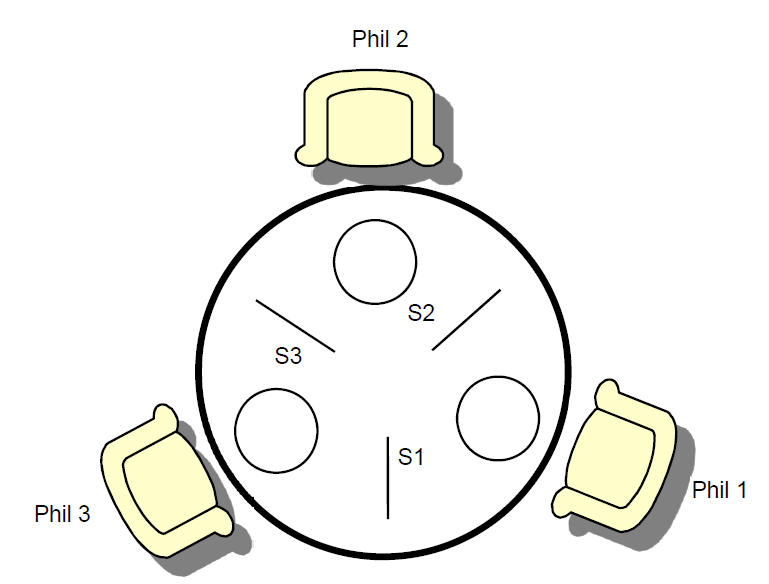
\includegraphics[width=.4\linewidth]{900-Praktika/prak05/pic.PNG}


\subsection{Aufgabe 1: Untersuchung von Deadlocks}
Untersuchen Sie die folgenden Fälle auf Verklemmungen (Deadlocks). Formulieren Sie eine verklemmungsfreie
Regel, bzw. welche der Varianten würden Sie implementieren? Die Regeln müssen so gestaltet werden,
dass die Philosophen während der "Synchronisation" ohne Absprachen untereinander auskommen, d.h.
bei Kenntnis dieser Regeln kann jeder Philosoph selbständig handeln.

\begin{enumerate}
  \item Jeder hungrige Philosoph nimmt seine beiden Stäbchen gleichzeitig auf, sobald beide verfügbar sind. Falls nur eines verfügbar ist, lässt er dieses auf dem Tisch liegen.
  \item Jeder hungrige Philosoph nimmt zuerst das Stäbchen links von seinem Teller auf. Das Stäbchen rechts von seinem Teller nimmt er nur dann auf, wenn er das linke schon hat.
  \item Alle Stäbchen werden durchnummeriert. Jeder hungrige Philosoph nimmt zuerst das Stäbchen mit der kleineren Nummer bei seinem Teller. Das Stäbchen mit der grösseren Nummer nimmt er nur dann auf, wenn er das Stäbchen mit der kleineren Nummer schon besitzt.
\end{enumerate}

\subsubsection{Lösung}

\begin{enumerate}
  \item Diese Variante funktioniert. Entweder nimmt der Philosoph gar kein Stäbchen oder zwei aufs Mal. Er muss einfach noch beide aufs Mal fassen können. Das könnte zu Problemen führen.
  \item Diese Variante funktioniert überhaupt nicht. Wenn alle Philosophen Hunger haben, nimmt jeder das linke Stäbchen und alle warten auf das zweite, welches aber keiner freigeben wird. Ein typischer Deadlock
  \item Diese Variante funktioniert, obwohl sie sehr ähnlich zu Variante b) aussieht. Die Regel gegen Deadlock lautet, dass alle die Ressourcen in der ganz genau gleichen Reihenfolge anfordern müssen. Zuerst links, dann rechts gemäss b) widerspricht dem. In b) will Phil 1 zuerst S1, dann S2, Phil 2 nimmt zuerst S2, dann S3, Phil 3 nimmt hingegen zuerst S3, dann S1. Hier liegt das Problem. In c) fordern Phil 1 und Phil 2 die Ressourcen genau gleich an wie in b). Phil 3 fordert aber zuerst S1 und dann S3 an, d.h. immer in derselben Reihenfolge.
\end{enumerate}

\subsection{Aufgabe 2: Implementation der dinierenden Philosophen}

m Verzeichnis ./Vorgabe/Philo finden Sie eine Codevorgabe für fünf Philosophen. Das main() ist sehr komfortabel: es müssen nur Objekte der Klasse Philosopher definiert werden. Diese Klasse bietet nur die beiden Elementfunktionen live() und join() an. Alles weitere, insbesondere die Erzeugung des Threadkontexts, ist intern in der Klasse umgesetzt. Studieren Sie den Code in Philosopher.h.

\begin{lstlisting}[language=C++, style=C++]
class Philosopher
{
  public:
    Philosopher(int pid, int thinkdelay, int eatDelay, Sticks& s);
    ~Philosopher();
    void live();       // the philosopher's life
    void join();       // wait for philosopher to leave
  private:
    enum {nMeals = 3};
    int id;            // this philosopher's id
    int tDelay;        // how long does this philosopher think?
    int eDelay;        // how long does this philosopher eat?
    int left;          // left fork number
    int right;         // right fork number
    Sticks& stick;     // sticks used by all philosophers
    pthread_attr_t attr;
    pthread_t tid;     // thread id
    void lifeThread(); // the (C++) - thread function
    static void* staticWrapper(void* p) // C Wrapper for pthread_create()
    {                                   // p must be the this pointer
        static_cast<Philosopher*>(p) -> lifeThread();
        return 0;
    }
};
\end{lstlisting}

\begin{enumerate}
  \item Erläutern Sie die Elementfunktion \texttt{Philosopher::lifeThread()}. Wozu dient sie?
  \item Erklären Sie die Funktion \texttt{Philosopher::staticWrapper()}. Wieso braucht es diese Funktion, was ist ihre Aufgabe und welche Beziehung hat diese Funktion zu \texttt{Philosopher::lifeThread()}?
  \item Schreiben Sie ein Programm in C++, welches das Philosophenleben simuliert und für alle fünf Philosophen gleich fair ist. Ein Deadlock darf nie eintreten. Implementieren Sie jeden Philosophen als Thread in\newline\texttt{Philosopher::live()}, die Denkphase können Sie mit einer jeweils zufällig gewählten Schlafdauer umsetzen. Den Zugriff auf die Stäbchen müssen Sie in der Klasse Sticks als Monitor implementieren, d.h. alle Locks müssen in dieser Klasse mit \texttt{pthread\_mutex\_lock()}, bzw. \texttt{pthread\_mutex\_unlock()} gemacht werden, der Aufrufer muss sich nicht darum kümmern müssen. Eine Condition Variable braucht es hier ebenfalls.
  \item In der Monitorklasse Sticks verwenden Sie bisher direkt die C-Funktionen \texttt{pthread\_mutex\_lock()}, bzw. \texttt{pthread\_mutex\_unlock()}. Setzen Sie jetzt RAII (Resource Acquisition Is Initialization) ein. Beachten Sie dazu auch die Klasse \texttt{ResourceLock} aus dem Praktikum 10 (Aufgabe 3) vom Modul Embedded Software Engineering 1.
\end{enumerate}

\subsubsection{Lösung}

\begin{enumerate}
  \item Die Elementfunktion \texttt{Philosopher::lifeThread()} ist die Threadfunktion, d.h. sie beinhaltet den Code, den ein Thread auszuführen hat. Sie hat den Zugriff auf sämtliche (auch privaten) Attribute und Funktionen der Klasse Philosopher. Sie zeigt, wie auch in C++ eine Elementfunktion als Threadfunktion genutzt werden kann.
  \item Ein Thread muss mit der C-Funktion \texttt{pthread\_create()} gestartet werden. Diese Funktion benötigt als Parameter einen Funktionspointer auf eine C-Funktion, welche die Threadfunktion beinhaltet. Die statische C++-Funktion \texttt{Philosopher::staticWrapper()} liegt ausserhalb des Klassenkontextes und kann der Funktion \texttt{pthread\_create()} übergeben werden. Der Static Wrapper ruft im Objektkontext die Elementfunktion \texttt{Philosopher::lifeThread()} auf. Den Objektkontext erhält der Wrapper über den void-Pointer. Deshalb muss der Funktion \texttt{pthread\_create()} der this-Pointer (das ist der Objektkontext) übergeben werden: \texttt{pthread\_create(\&tid, \&attr, staticWrapper, this);}
  \item siehe ./Loesung/Philo Bei der Ausführung bemerken Sie allenfalls, dass cout nicht thread-safe ist. Einzelne Texte mögen auseinandergerissen (interleaved) sein.

\lstinputlisting[language=C++, style=C++, multicols=2]{900-Praktika/prak05/Loesung/Philo/sticks.h}
\noindent\makebox[\linewidth]{\rule{\paperwidth}{0.4pt}}
\lstinputlisting[language=C++, style=C++, multicols=2]{900-Praktika/prak05/Loesung/Philo/sticks.cpp}
\noindent\makebox[\linewidth]{\rule{\paperwidth}{0.4pt}}
\lstinputlisting[language=C++, style=C++, multicols=2]{900-Praktika/prak05/Loesung/Philo/Philosopher.h}
\noindent\makebox[\linewidth]{\rule{\paperwidth}{0.4pt}}
\lstinputlisting[language=C++, style=C++, multicols=2]{900-Praktika/prak05/Loesung/Philo/Philosopher.cpp}
\noindent\makebox[\linewidth]{\rule{\paperwidth}{0.4pt}}
\lstinputlisting[language=C++, style=C++, multicols=2]{900-Praktika/prak05/Loesung/Philo/PhiloTest.cpp}

  \item siehe ./Loesung/PhiloRAII Sie benötigen die Klasse ResourceLock. Ein Objekt dieser Klasse müssen Sie in den beiden Elementfunktionen \texttt{Sticks::get()} und \texttt{Sticks::put()} einsetzen. Der Rest bleibt sich gleich.
\end{enumerate}

\lstinputlisting[language=C++, style=C++, multicols=2]{900-Praktika/prak05/Loesung/PhiloRAII/ResourceLock.h}
\noindent\makebox[\linewidth]{\rule{\paperwidth}{0.4pt}}
\lstinputlisting[language=C++, style=C++, multicols=2]{900-Praktika/prak05/Loesung/PhiloRAII/sticks.h}
\noindent\makebox[\linewidth]{\rule{\paperwidth}{0.4pt}}
\lstinputlisting[language=C++, style=C++, multicols=2]{900-Praktika/prak05/Loesung/PhiloRAII/sticks.cpp}
\noindent\makebox[\linewidth]{\rule{\paperwidth}{0.4pt}}
\lstinputlisting[language=C++, style=C++, multicols=2]{900-Praktika/prak05/Loesung/PhiloRAII/Philosopher.h}
\noindent\makebox[\linewidth]{\rule{\paperwidth}{0.4pt}}
\lstinputlisting[language=C++, style=C++, multicols=2]{900-Praktika/prak05/Loesung/PhiloRAII/Philosopher.cpp}
\noindent\makebox[\linewidth]{\rule{\paperwidth}{0.4pt}}
\lstinputlisting[language=C++, style=C++, multicols=2]{900-Praktika/prak05/Loesung/PhiloRAII/PhiloTest.cpp}

\newpage
\section{Lab 6 CRC - Berechnung und -Implementation in C++}
%!TEX root = ../prak.tex
\section{Lab 6 CRC - Berechnung und -Implementation in C++}
\subsection{Aufgabe 1: CRC-8 Berechnungsbeispiel (Papierübung)}
Berechnen Sie die Checksumme für den unten abgebildeten Bytestream. Verwenden Sie dafür das Generatorpolynom
$G = x^8 + x^2 + x + 1$ (entspricht CRC-8 CCITT).

Message : 00101101 = 0x2D

\subsubsection{Lösung}
\begin{center}
  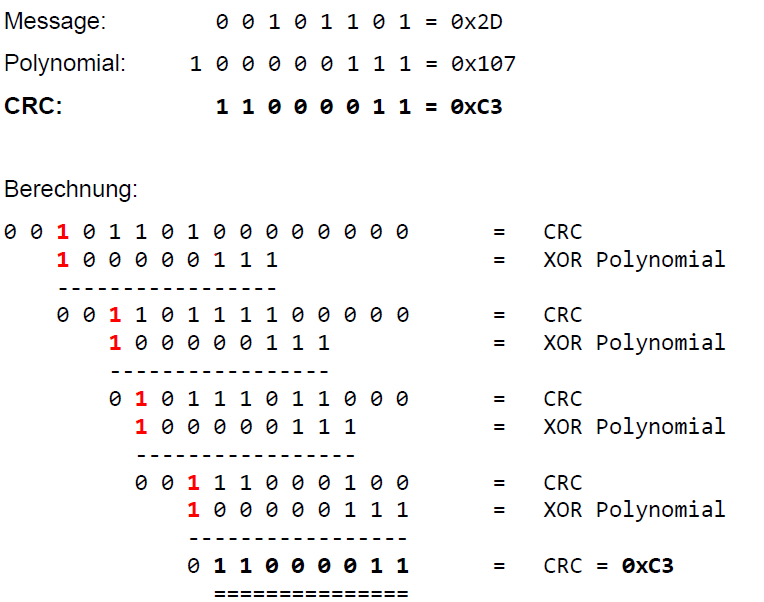
\includegraphics[width=.5\linewidth]{900-Praktika/prak06/crc1.PNG}
\end{center}

\subsection{Aufgabe 2: Verifikation empfangener Daten mittels CRC}

Nach einer seriellen Übertragung wurden die folgenden drei Messages empfangen. Dabei entspricht das erste Byte den \textcolor{blue}{Daten} und das zweite der \textcolor{orange}{CRC-Prüfsumme} (MSB first). Das verwendete Generatorpolynom ist dasselbe wie in Aufgabe 1 (CRC-8 CCITT).

Überprüfen Sie, welche der drei Messages fehlerfrei übertragen wurden und welche nicht.

\subsubsection{Lösung}
\begin{center}
  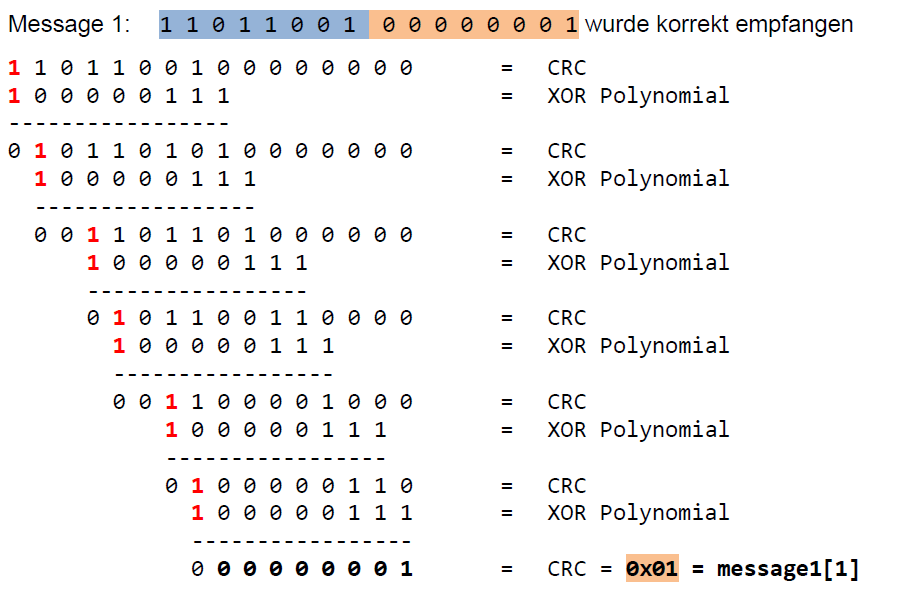
\includegraphics[width=.6\linewidth]{900-Praktika/prak06/crc2.PNG}
\end{center}

Bei der noch einfacheren Möglichkeit zur Verifikation werden die gesamten empfangenen Daten inklusive der Prüfbits durch das Generatorpolynom gelassen. Wenn alles korrekt ist, so muss am Schluss der Wert 0 als CRC übrigbleiben

\begin{center}
  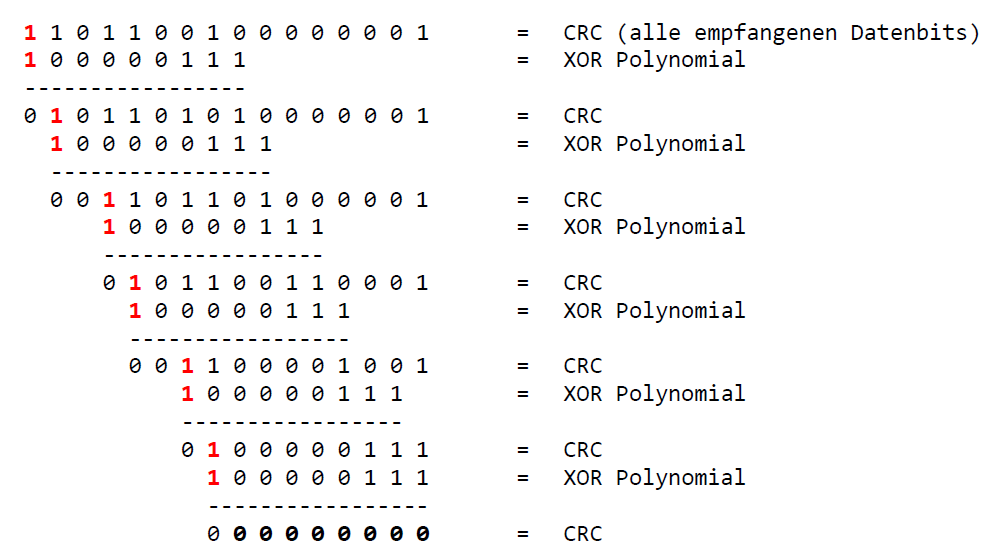
\includegraphics[width=.6\linewidth]{900-Praktika/prak06/crc3.PNG}
  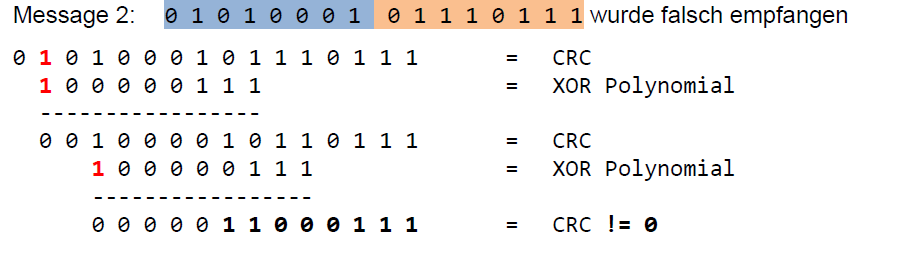
\includegraphics[width=.6\linewidth]{900-Praktika/prak06/crc4.PNG}
  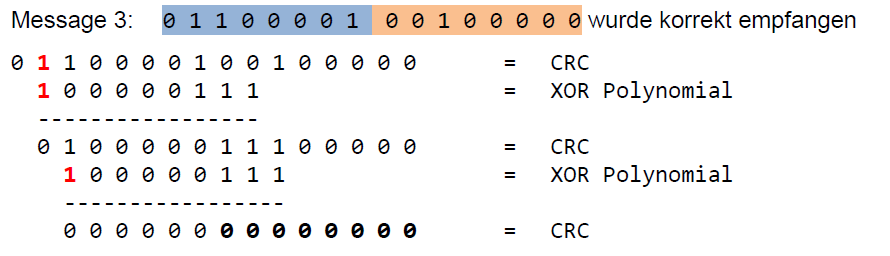
\includegraphics[width=.6\linewidth]{900-Praktika/prak06/crc5.PNG}
\end{center}

Die zweite Message wurde falsch empfangen. Entweder ist das Daten- oder das Prüfsummenbyte korrupt. Der Empfänger muss in einem solchen Fall ein NAK zurückgeben, um die Message noch einmal anzufordern.

\subsection{Aufgabe 3: C++ - Implementation}
Implementieren Sie eine Klasse Crc, welche die Prüfsumme CRC-8 CCITT mit Schiebeoperationen auf Bit-Ebene berechnet. Um den Algorithmus zu überprüfen, soll ein Testprogramm geschrieben werden, welches entweder die Prüfsumme der Datenbytes aus Aufgabe 2 berechnet, oder die Prüfsumme der vorgegebenen Datei ausgibt. Der Dateiname soll der Applikation als Argument übergeben werden.

\subsubsection{Lösung}

Wird das Programm ohne Argument aufgerufen, berechnet es die Prüfsumme von {0xd9, 0x51, 0x61}.

\begin{lstlisting}[language=C++, style=C++]
$ ./crcTest
CRC-8 CCITT Bit um Bit, einfach aber ineffizient

CRC-8 CCITT der einzelnen Datenbytes:
Byte 00: crc(0xd9) = 0x01
Byte 01: crc(0x51) = 0xb0
Byte 02: crc(0x61) = 0x20
CRC-8 CCITT von allen Datenbytes:
crc(0xd95161) = 0x2c
\end{lstlisting}

Mit einem gültigen Dateinamen als Argument wird diese Datei in einen Byte-Buffer gelesen und die Prüfsumme über den gesamten Buffer berechnet.

\begin{lstlisting}[language=C++, style=C++]
$ ./crcTest datafile.txt
CRC-8 CCITT Bit um Bit, einfach aber ineffizient

Datei: datafile.txt
Anzahl Datenbytes: 72125
CRC-8 CCITT: 0x10
\end{lstlisting}

\lstinputlisting[language=C++, style=C++, multicols=2]{900-Praktika/prak06/Loesung/A3/Crc.h}
\noindent\makebox[\linewidth]{\rule{\paperwidth}{0.4pt}}
\lstinputlisting[language=C++, style=C++, multicols=2]{900-Praktika/prak06/Loesung/A3/Crc.cpp}
\noindent\makebox[\linewidth]{\rule{\paperwidth}{0.4pt}}
\lstinputlisting[language=C++, style=C++, multicols=2]{900-Praktika/prak06/Loesung/A3/CrcTest.cpp}

\subsection{Aufgabe 4: C++ - Implementation mit einer Lookup Tabelle}
Implementieren Sie eine Klasse Crc, welche die Prüfsumme CRC-8 CCITT mit Hilfe einer 8 Bit breiten Lookup Tabelle berechnet. Die Lookup Tabelle kann im Voraus berechnet werden oder sogar konstant im ROM abgelegt werden. Um den Algorithmus zu überprüfen soll ein Testprogramm geschrieben werden, welches entweder die Prüfsumme der Datenbytes aus Aufgabe 2 berechnet, oder die Prüfsumme der vorgegebenen Datei ausgibt. Der Dateiname soll der Applikation als Argument übergeben werden. Variieren Sie die Dateigrösse und vergleichen Sie die Berechnungszeit mit der Variante aus der Aufgabe 3.

\medskip

Hinweis File I/O:

\begin{lstlisting}[language=C++, style=C++]
#include <fstream>
// ...
f.open(argv[1], ios::in | ios::binary);
// determine file size
f.seekg(0, ios::end);
len = f.tellg();
f.seekg(0, ios::beg);
// Allocate byte buffer
buf = new uint8_t[len];
// read file content into byte buffer
f.read((char*)buf, len);
f.close();
// ...
delete[] buf; // free allocated memory
\end{lstlisting}

\subsubsection{Lösung}


\lstinputlisting[language=C++, style=C++, multicols=2]{900-Praktika/prak06/Loesung/A4/Crc.h}
\noindent\makebox[\linewidth]{\rule{\paperwidth}{0.4pt}}
\lstinputlisting[language=C++, style=C++, multicols=2]{900-Praktika/prak06/Loesung/A4/Crc.cpp}
\noindent\makebox[\linewidth]{\rule{\paperwidth}{0.4pt}}
\lstinputlisting[language=C++, style=C++, multicols=2]{900-Praktika/prak06/Loesung/A4/CrcTest.cpp}

\subsection{Aufgabe 5: Callgrind}
Mit dem Tool Callgrind kann die Laufzeit eines Programms analysiert werden. In der Standardkonfiguration werden die Anzahl der ausgeführten Instruktionen aufgezeichnet. Die aufgezeichnete Anzahl der Instruktionen wird zudem mit Sourcecode-Zeilen und Funktionsaufrufen in Beziehung gesetzt. Zusätzlich kann eine Cachesimulation aktiviert werden, die weitere Informationen über die Laufzeitperformance des Programms geben kann. Die Cachesimulation führt das gleiche aus wie das Tool Cachegrind. Callgrind schreibt das Ergebnis der Laufzeitanalyse in eine Datei. Die Datei kann dann mit dem Programm KCachegrind visualisiert werden.
In dieser Aufgabe sollen Sie die CRC-8 CCITT Implementationen mittels Tabelle und mittels Schiebeoperationen auf Bit-Ebene mit Valgrind profilen.

Beachten Sie die Vorgabe und binden Sie Ihre eigenen CRC-Implementationen ein.

Callgrind: Profilen Sie die beiden CRC Implementationen mit dem Tool Callgrind. Visualisieren sie die Ausgabe mit KCachegrind und untersuchen sie die Performanceunterschiede.
\begin{enumerate}
  \item In welchem Sourcecode-File liegt der Hotspot. Auf welchen Sourcecode-Zeilen liegt der Hotspot im entsprechenden File für die CRC-Berechnung? Wie unterscheiden sich die beiden Implementationen bezüglich Laufzeitperformance?
  \item Wie verändert sich die Performance der beiden Programme, wenn mit Optimierungsstufe –O3 kompiliert wird? Verändert sich der Hotspot der beiden CRC-8 Implementationen gleichermassen mit eingeschalteter Optimierung?
\end{enumerate}

\textbf{Hinweis:} Übergeben Sie für das Callgrind-Profiling das datafile.txt dem CRC Testprogramm, damit der CRC über einige Bytes berechnet werden muss und dadurch der Overhead für Systemfunktionen bezogen auf die CRC Berechnung kleiner wird.

\subsubsection{Lösung}

Die verwendeten Profiling-Befehle finden Sie in den make-Files in ./Loesung/A5.

\begin{enumerate}
  \item Bei beiden Implementationen benötigt die Funktion \texttt{Crc::getCrc()} aus crc.cpp am meisten Rechenzeit. In dieser Funktion liegt der Hotspot bei der for-Schleife. Der Unterschied der beiden Implementationen kann an der Anzahl Zyklen festgestellt werden. Bei der Tabellenimplementation werden 1‘442‘513 Zyklen und bei der Schiebeoperationsvariante 7‘571‘101 Zyklen verbraucht. Daraus geht hervor, dass die Tabellenvariante etwa 5.2-mal schneller ist als die Schiebeoperationsvariante.

  \lstinputlisting[language=C++, style=C++, multicols=2]{900-Praktika/prak06/Loesung/A5/CrcBitWise/makefile}

  \item Die Schiebeoperationsvariante reduziert die Anzahl der Zyklen um 70 \% auf 2‘235‘591 Zyklen und die Tabellenvariante ebenfalls um 70 \% auf 432‘757 Zyklen.

  \lstinputlisting[language=C++, style=C++, multicols=2]{900-Praktika/prak06/Loesung/A5/CrcBitWiseO3/makefile}

\end{enumerate}

\newpage
\section{Lab 7 inline und Bitfelder}
%!TEX root = ../prak.tex
\section{Lab 7 inline und Bitfelder}
\textbf{Allgemeine Bemerkungen zu Effizienz- und Performancebetrachtungen:}
Die Effizienz- und Performancebetrachtungen sind stark von der Qualität des Compilers abhängig. Die aktuelle Version des GNU-Compilers (Version 7.4.0) erzeugt sehr effizienten Code, da die Link-Time Optimization eingeführt wurde. Im Gegensatz zur Compile-Time Optimization wird der aus den einzelnen Objectfiles gelinkte Programmcode als Ganzes analysiert und optimiert.
Die folgenden Optionen der GNU-Compiler könnten nützlich sein:

\medskip
\noindent
-E \qquad Precompile only, der Output wird auf stdout geschrieben \\
-S \qquad Assembleroutput, ohne Objectfile erzeugen\\
-c \qquad nur compilieren\\
-O0 \quad keine Optimierung\\
-O1 \quad Optimierungsstufe 1 (siehe g++ $--$help für Details)\\
-O2 \quad Optimierungsstufe 2\\
-O3 \quad Optimierungsstufe 3\\
-Os \quad Optimierung auf Codegrösse\\

Hinweise zum x86-Instruktionssatz finden Sie unter anderem im Manual 64-ia-32-architectures-software-developer-manual-325462.pdf und auf folgenden Websites:

\url{http://en.wikipedia.org/wiki/X86_instruction_listings}

\url{http://www.cs.uaf.edu/2005/fall/cs301/support/x86/index.html}

\url{http://ref.x86asm.net/}

\subsection{Aufgabe 1: inline-Methoden}

Bei sehr kurzen Methoden (Einzeiler) ist der Overhead eines Funktionsaufrufs recht gross. Durch Inlining kann der Funktionsaufruf vermieden werden, der Code (Funktionsrumpf) wird vom Compiler direkt anstelle des Funktionsaufrufs gesetzt. Der Compiler wird üblicherweise keinen Inlinecode erzeugen, falls die Funktion rekursiv aufgerufen wird oder falls ein Pointer auf diese Funktion verwendet wird. Eine weitere Schwierigkeit ergibt sich, wenn die Inlinefunktionen in mehreren Sourcefiles verwendet werden sollen, der Linker kann aus einer bestehenden Objektdatei kaum Inlinecode erzeugen.

Für diese Aufgabe ist zusätzlich die folgende Option der GNU-Compiler nützlich:

\texttt{-Winline} Erzeugt eine Warnung, falls von einer mit inline spezifizierten Funktion kein Inlinecode erzeugt werden konnte.
Verwenden Sie für diese Untersuchungen die Linux-Konsole im Ubuntu-Image, Eclipse bietet keine Vorteile.

\begin{enumerate}
  \item Wenn bei Klassendeklarationen der Code direkt definiert wird, sind diese Funktionen implizit inline. Verwenden Sie den im Verzeichnis ./Vorgabe/Rectangle zur Verfügung gestellte C++-Code. Wie Sie feststellen, ist die Methode getArea() nicht inline. Compilieren Sie dieses Programm, ein Makefile steht zur Verfügung.
  \item Betrachten Sie die erzeugten Assemblerfiles. Welche Methoden sind inline, welche nicht? Hinweis: betrachten Sie dazu die call-Befehle.
  \item Wenn Sie die einzelnen *.s-Dateien betrachten, können Sie nicht feststellen, ob der Linker allenfalls auch noch optimieren kann. Relevant ist einzig, wie der Code in der Programmdatei aussieht. Verwenden sie den Debugger gdb von der Kommandozeile, um dies festzustellen. Starten Sie die Debugsession mit dem Befehl gdb ./main. Anschliessend müssen Sie das Programm starten mit start. Den disassemblierten Code sehen Sie, wenn Sie disassem eintippen. Im Folgenden sehen Sie den Ausschnitt einer Debugsession.

\begin{lstlisting}[language=C++, style=C++]
gdb ./main
  GNU gdb (Ubuntu 8.1-0ubuntu3.2) 8.1.0.20180409-git
  ...
  (gdb) start
  Temporary breakpoint 1 at 0x66e
  ...
  Temporary breakpoint 1, 0x000055555555466e in main ()
  (gdb) disassem
  Dump of assembler code for function main:
    0x000055555555466a <+0>:  push   %rbp
    0x000055555555466b <+1>:  mov    %rsp,%rbp
  => 0x000055555555466e <+4>: sub    $0x40,%rsp
  ...
\end{lstlisting}

  \item Wahrscheinlich haben Sie festgestellt, dass alle Methoden mit einem Call aufgerufen werden. Ändern Sie die Optimierungsstufe bis alle Methoden ausser getArea() inline sind.
  \item Sie möchten nun sowohl die impliziten Inlinefunktionen ins cpp-File zügeln, als auch von getArea() Inlinecode erhalten. Sie müssen die Funktionen mit inline kennzeichnen. Häufig werden die Implementationen der Inlinefunktionen direkt unter die Klassendeklaration verschoben.
  \item Testen Sie, ob alles richtig funktioniert, indem Sie ein Projekt mit mehreren cpp-Files erstellen, welche die Inlinefunktionen verwenden, d.h. main.cpp plus ein weiteres File. Betrachten Sie die Assemblerfiles, es sollte keine Calls auf Memberfunktionen mehr geben.
\end{enumerate}

\subsubsection{Lösung}

\begin{enumerate}
  \item just do it
  \item Bei Optimierungsstufe 0 sind keine Funktionen inline (siehe ./Loesung/A1-b). Man erkennt das daran, dass bei den einzelnen Funktionen Labels definiert sind und mit einem Return (\texttt{ret}) abgeschlossen werden. Die Funktionen werden mit einem \texttt{call}-Befehl aufgerufen (siehe folgenden Ausschnitt)

\begin{center}
  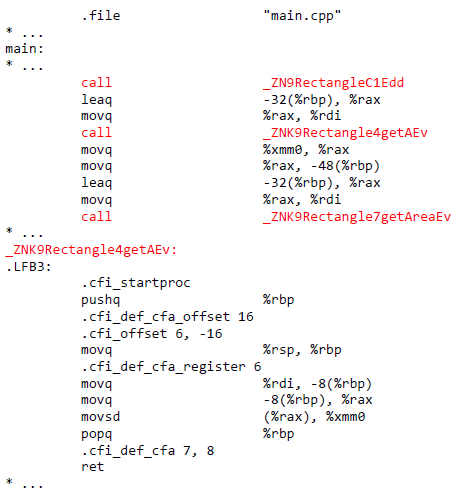
\includegraphics[width=.5\linewidth]{900-Praktika/prak07/1.PNG}
\end{center}

  \item Der Debugger-Output zeigt, dass bei Optimierungsstufe 0 alle Funktionen mit call aufgerufen werden.

\begin{center}
  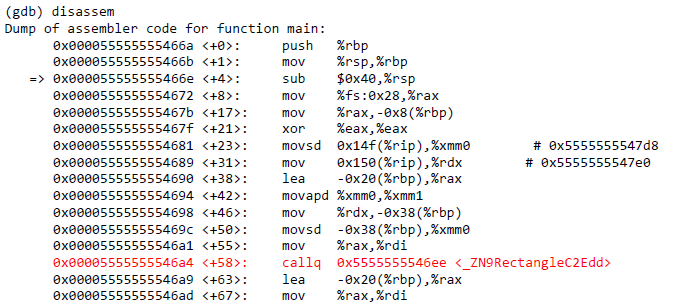
\includegraphics[width=.8\linewidth]{900-Praktika/prak07/2.PNG}
  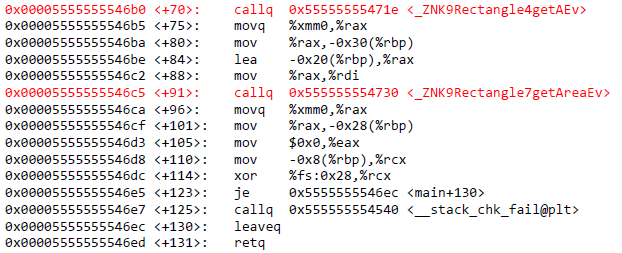
\includegraphics[width=.8\linewidth]{900-Praktika/prak07/3.PNG}
\end{center}

  \item Ab Optimierungsstufe 1 sind die impliziten inline-Funktionen alle inline, auch der Konstruktor (siehe Zeile 0x00005555555546a4 $<$+58 $>$: in Aufgabe c). Einzig die Funktion \texttt{getArea()} wird immer noch aufgerufen, da diese Funktion in einer anderen Objectdatei liegt (siehe ./Loesung/A1-d/*.s). Der Assemblerdump zeigt das:

\begin{center}
  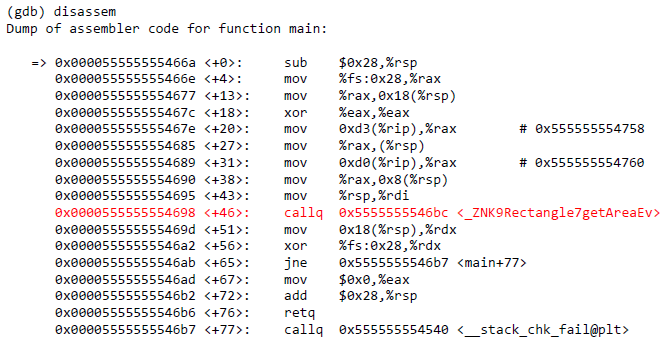
\includegraphics[width=.8\linewidth]{900-Praktika/prak07/4.PNG}
\end{center}

  \item Wenn das bestehende \texttt{main()} genommen wird, so optimiert der Compiler ab Optimierungsstufe 1 alle Variablen weg, da sie nicht verwendet werden (siehe ./Loesung/A1-e1/main.s).

\begin{center}
  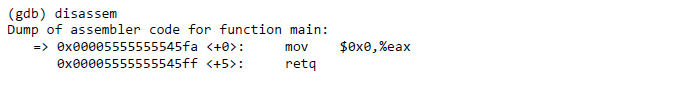
\includegraphics[width=.8\linewidth]{900-Praktika/prak07/7.PNG}
\end{center}

  In der beiliegenden Lösung (siehe ./Loesung/A1-e2) werden die Daten deshalb auf cout geschrieben oder die Variablen als volatile deklariert, d.h. die Berechnungen können nicht wegoptimiert werden. Die Methoden können bei der Deklaration, bei der Definition oder bei beiden Stellen mit inline gekennzeichnet werden.
  \item siehe ./Loesung/A1-f Eine neue Funktion \texttt{getRectangleB(const Rectangle\& r)} wurde im File rectangleB.cpp eingeführt. Die Funktion verwendet inline Methoden der Rectangle-Klasse um b zu berechnen. Im gdb-Dump kann nachgeprüft werden dass im main nur ein einziger Call vorkommt (\texttt{getRectangleB())}:

\begin{center}
  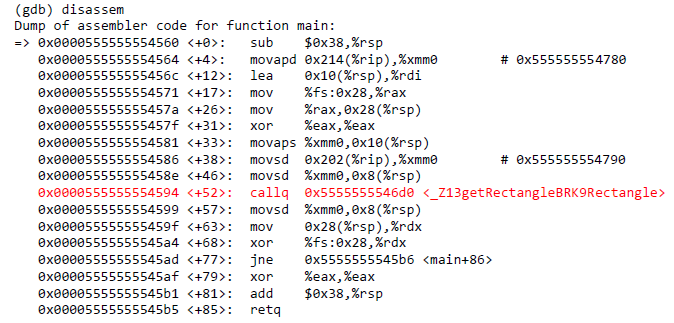
\includegraphics[width=.8\linewidth]{900-Praktika/prak07/5.PNG}
\end{center}

  Zudem darf in der Funktion \texttt{getRectangleB()} kein Call vorkommen, da die verwendeten Methoden inline sein müssen:

\begin{center}
  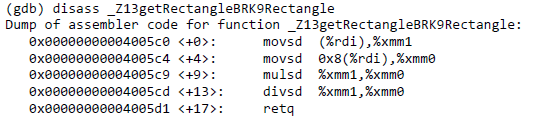
\includegraphics[width=.8\linewidth]{900-Praktika/prak07/6.PNG}
\end{center}

\end{enumerate}

\subsection{Aufgabe 2: Bitfelder}

Gegeben ist das nachfolgende Register

\begin{center}
  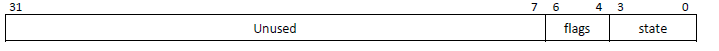
\includegraphics[width=.8\linewidth]{900-Praktika/prak07/bitmuster.PNG}
\end{center}


\begin{enumerate}
  \item Definieren Sie dieses Register mit Hilfe eines Bitfelds. Die Variable (z.B. r) müssen Sie mit volatile kennzeichnen. Wieso?
  \item Setzen Sie nun state auf den Wert 15 und flags auf den Wert 3. Untersuchen Sie, wie der Assembler-code aussieht.
  \item Inkrementieren Sie nun flags mittels ++r.flags. Achten Sie nun auf den Code.
  \item Führen Sie mit flags eine übliche Bitoperation durch, z.B. r.flags \&= 6. Achten Sie nun auf den Code.
  \item Diskutieren Sie die erhaltenen Ergebnisse. Entspricht das Resultat Ihren Erwartungen? Worüber sind Sie überrascht? Sollen Bitfelder so verwendet werden? Sollen sie überhaupt verwendet werden?
\end{enumerate}

\subsubsection{Lösung}

\begin{enumerate}
  \item volatile muss verwendet werden, weil die Variable auf ein Hardwareregister gemappt wird und nicht wegoptimiert werden darf. Zudem können die Werte von Registern ebenfalls durch die Hardware geändert werden. Deshalb muss der Code so generiert werden, dass das Register jedesmal zuerst gelesen wird bevor damit gearbeitet wird. Wenn dies nicht gemacht würde, könnte passieren, dass mit einer Kopie des Registerinhalts gearbeitet wird, der in der Zwischenzeit durch die Hardware geändert wurde.
  \lstinputlisting[language=C++, style=C++, multicols=2]{900-Praktika/prak07/Loesung/A2/main.s}

  \item Die Registervariable wird auf -4(\%ebp) gelegt, d.h. auf den Stack. Aus dem Zugriff auf state wird direkt eine OR-Operation (orl). Da die Variable volatile ist, werden die Werte laufend zwischen dem Stack und dem Register eax hin- und hergeschoben. Der Wert auf dem Stack muss immer der richtige und aktuelle sein.
\begin{lstlisting}[language=C++, style=C++]
movl     $0, -4(%rsp)
...
movl     -4(%rsp), %eax
orl      $15, %eax
movl     %eax, -4(%rsp)
\end{lstlisting}
  Das direkte Setzen von flags wird ebenfalls in eine OR-Operation umgewandelt, wobei die flags-Bits zuerst ausmaskiert werden (andl \$-113,\% eax).
\begin{lstlisting}[language=C++, style=C++]
movl    -4(%rsp), %eax
andl    $-113, %eax
orl     $48, %eax
movl    %eax, -4(%rsp)
\end{lstlisting}
  \item Beim Inkrementieren von flags wird mit Schiebeoperationen (zuerst nach rechts, dann nach links) und den Registern A und D gearbeitet. Dieser Zugriff wird sehr ineffizient.
\begin{lstlisting}[language=C++, style=C++]
movl       -4(%rsp), %eax
movl       -4(%rsp), %edx
shrl       $4, %eax
addl       $1, %eax
andl       $-113, %edx
andl       $7, %eax
sall       $4, %eax
orl%edx,   %eax
movl       %eax, -4(%rsp)
\end{lstlisting}
\textbf{Pseudocode:}
\begin{enumerate}
  \item  Wert von r in die Register A und D kopieren
  \item Register D um 4 Bits nach rechts schieben, um eins Inkrementieren, mit 7 ausmaskieren und wieder um 4 Bits nach links schieben
  \item Flags-Bits in Register A ausmaskieren und mit Register D verodern
  \item Register A in r speichern
\end{enumerate}
\textbf{Hinweis für den Registerzugriff (Beispiel Register D):}

\begin{lstlisting}[language=C++, style=C++]
|63..32|31..16|15-8|7-0|
               |DH.|DL.| <- DH / DL adressieren das High- / Low-Byte der untern 16
                            Bits von Register D
               |DX.....| <- adressiert die unteren 16 Bits von Register D
       |EDX............| <- EDX adressiert die unteren 32 Bits von Register
|RDX...................| <- RDX adressiert alle 64 Bits von Register D
\end{lstlisting}
  \item Auch die Operation r.flags \&= 6 wird sehr ineffizient durchgeführt, da das Muster zuerst an Bitposition 0 geschoben wird, dann wird die Operation durchgeführt und abschliessend wieder zurückgeschoben.
  \item Bitfelder sind bekanntlich nicht standardisiert. Wenn die einzelnen Felder direkt gesetzt werden, dann erzeugt der GNU-Compiler effizienten Code, er nimmt direkt eine Bitoperation. Wenn hingegen Operationen durchgeführt werden wie r.flags \&= 6, dann wird sehr ineffizienter Code generiert. Die meisten anderen Compiler können das auch nicht besser. Bitfelder sollten deshalb aus meiner Sicht nicht verwendet werden, da nebst der nicht vorhandenen Portabilität zudem sehr ineffizienter Code entsteht.

\end{enumerate}

\subsection{Aufgabe 3: Bitmasken}
\begin{enumerate}
  \item Lösen Sie die Aufgabe 3 mit allen Operationen ausser der Addition direkt mittels (inline-) Operationen mit Bitmasken. Vergleichen Sie nun den Assemblercode mit dem Code aus Aufgabe 3.
  \item  Welche Erkenntnisse haben Sie aus den Resultaten der Aufgaben 3 und 4 gewonnen?
\end{enumerate}

\subsubsection{Lösung}

\begin{enumerate}
  \item Bei dieser Variante entsteht sehr effizienter Code. Eine Anweisung wie r \&= 6 $<<$ 4; wird direkt in ein AND umgewandelt, die Operation 6 $<<$ 4 berechnet der Compiler, nicht das Laufzeitsystem:
\begin{lstlisting}[language=C++, style=C++]
movl       $0, -4(%rsp)
movl       $15, -4(%rsp)
movl       -4(%rsp), %eax
orl        $48, %eax
movl       %eax, -4(%rsp)
movl       -4(%rsp), %eax
andl       $96, %eax
movl       %eax, -4(%rsp)
\end{lstlisting}
  \item  Bitmasken verwenden, Bitfelder nicht.


\end{enumerate}

\newpage
\section{Lab 8 Digitale Ableitung und Pulsdetektion auf dem EmbSW-Roboter}
In diesem Praktikum soll eine EKG-Messung auf dem EmbSW-Roboter verarbeitet werden. Das Ziel ist, eine
robuste Detektion der Herzpulse zu implementieren, damit der korrekte Puls auf der PC-Software angezeigt
wird.

\medskip
\textbf{Systemübersicht}
\medskip

Die EKG-Messdaten werden vom PC einzeln über die serielle Schnittstelle auf die Hardware übertragen. Jedes
Sample wird durch den Aufruf von \texttt{Ecg::processSample()} sofort verarbeitet, nachdem es vollständig
empfangen wurde. Anschliessend wird es mit der detektierten Phase des Herzpulses zu einem Telegramm
zusammengepackt und wieder an die PC-Software zurückgeschickt. Der Signalflussplan ist in Abbildung 1
dargestellt.

\begin{center}
  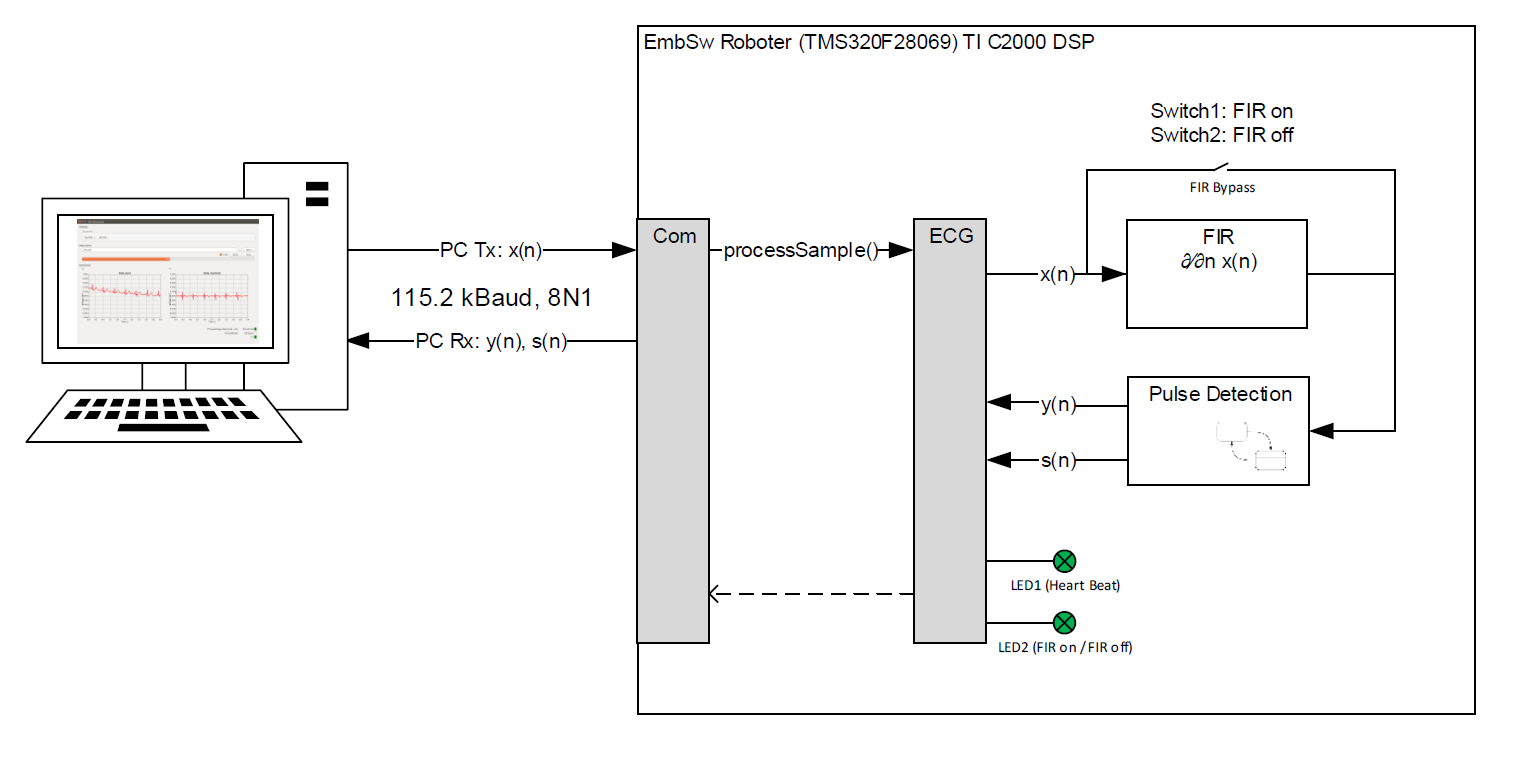
\includegraphics[width=.8\linewidth]{900-Praktika/prak08/1.PNG}
\end{center}

Die einzelnen Verarbeitungsblöcke (hier FIR und Pulse Detection) sind seriell zusammengeschaltet und können
ein- bzw. ausgeschaltet werden. Mit dem Switch1 auf dem Roboter kann das FIR-Filter eingeschalten
bzw. mit Switch2 wieder ausgeschalten werden.

\medskip
\textbf{Klassendiagramm der Vorgabe}

Das Vorgabeprojekt besteht aus den Klassen Ecg, Fir und PulseDetection. Zudem wird der Unit Test für
diese Einheit zur Verfügung gestellt.
Die Datenverarbeitung startet mit dem Aufruf von \texttt{Ecg::processSample()}. Die Klasse Ecg beinhaltet ein
Array von Algorithmen, die für jedes Sample der Reihe nach abgearbeitet werden. Der neu berechnete Wert
und ein detektierter Herzschlag wird schliesslich von der Funktion \texttt{Ecg::processSample()} zurück gegeben.
Alle Algorithmen besitzen dieselbe Basisklasse Algorithm. In den Unterklassen muss die virtuelle Funktion
\texttt{Algorithm::process(float, float\&)} überschrieben werden, um die nötige Funktion zu implementieren.
Wird diese Funktion von der abgeleiteten Klasse nicht überschrieben, so hat dieser Algorithmus keinen Einfluss
auf die Signalverarbeitung, da der Ausgangswert gleich dem Eingangswert gesetzt wird.
\begin{center}
  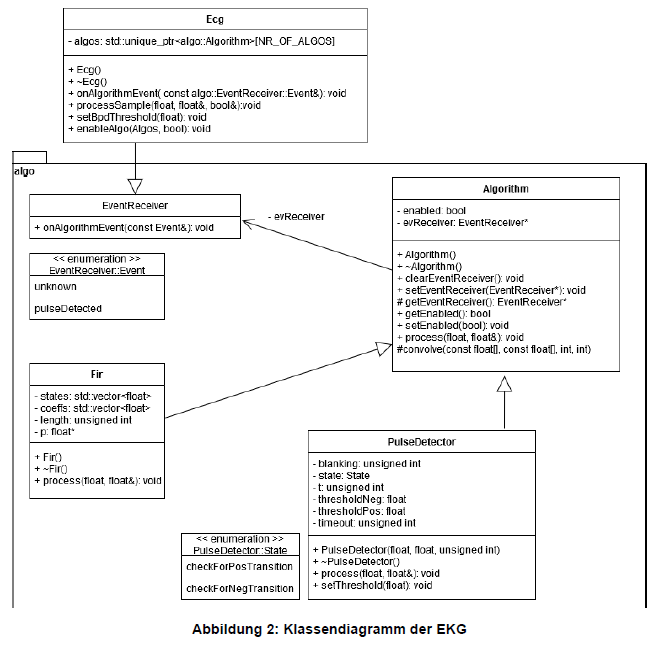
\includegraphics[width=1\linewidth]{900-Praktika/prak08/2.PNG}
\end{center}

\subsection{Aufgabe 1: Implementation des FIR-Filters}
Für eine robuste Detektion der Herzpulse soll das EKG-Signal zuerst über einen geeigneten Filter abgeleitet werden. Der Filter wird in Form eines FIR-Filters implementiert und erbt von der Klasse Algorithm. Die ein-fachste Variante wäre ein Filter mit den Koeffizienten $[1 -1]$, was einem Differenziator entspricht. Das Aus-gangssignal berechnet sich nach: $y[n] = 1\cdot x[n] – 1 \cdot x[n-1]$;
Dieses Filter reagiert stark auf die Rauschkomponente des Signals und liefert eine unbrauchbare Ableitung. Besser ist es, die Ableitung mit einer gleichzeitigen Bandpass-Filterung zu kombinieren. Eine Möglichkeit dafür ist das Savitzky-Golay-Filter (Savitzky \& Golay, 1964). Eine Analyse in MATLAB zeigt, dass eine Fen-sterbreite von 5 Samples und eine Ordnung von 3 eine optimale Ableitung generiert. Die resultierenden Ko-effizienten sind unten abgebildet.

\texttt{static const float sgFilterCoeffs[] = \{ 0.0833, -0.6667, 0.0000, 0.6667, -0.0833 \};}

\begin{enumerate}
  \item Definieren Sie die oben erwähnten Koeffizienten in der Klasse Ecg.
\item  Vervollständigen Sie die Methode process() der Klasse FIR indem Sie ein FIR-Filter implementieren. Mögliche Implementationen finden Sie im Buch \textit{Introduction to Signal Processing} von Sophocles J. Or-fanidis, Kapitel 4.2.4 \textit{Hardware Realizations and Circular Buffers}.
\item Testen Sie die korrekte Funktion mit dem Test Case FirTest des ECG Unit Tests. (Hinweis: Test Case PulseDetectorTest kann für diese Aufgabe auskommentiert werden.)
\end{enumerate}

\subsubsection{Lösung}

\begin{enumerate}
  \item siehe Eclipse-Projekt in ./Loesung/Ecg/, im speziellen die Klassen ./Loesung/Ecg/algo/FIR.cpp und Filterkoeffizienten in ./Loesung/Ecg/Ecg.cpp:
\texttt{const float Ecg::sgFilterCoeffs[] = \{0.0833, -0.6667, 0.0, 0.6667, -0.0833\};}
Die Implementation des FIR Filters ist für das bessere Verständnis sehr allgemein gehalten. Die Basis der Implementation stammt vom Buch \textit{Introduction to Signal Processing} von Sophocles J. Orfanidis, Kapitel 4.2.4 \textit{Hardware Realizations and Circular Buffers}.
Für den verwendeten DSP gibt es eine Implementation eines FIR Filters von TI selbst in einer DSP-Lib-rary. Zu empfehlen sind die DSP Algorithmus-Implementationen von den Herstellern, da sie meistens sehr effizient codiert sind.
\item Die Unit Test Cases \texttt{DisabledTest} und \texttt{FirTest} muss fehlerfrei ausgeführt werden können. Siehe Eclipse-Projekt in ./Loesung/Ecg
\end{enumerate}

\lstinputlisting[language=C++, style=C++, multicols=2]{900-Praktika/prak08/Loesung/Ecg/Ecg.h}
\noindent\makebox[\linewidth]{\rule{\paperwidth}{0.4pt}}
\lstinputlisting[language=C++, style=C++, multicols=2]{900-Praktika/prak08/Loesung/Ecg/Ecg.cpp}
\noindent\makebox[\linewidth]{\rule{\paperwidth}{0.4pt}}
\lstinputlisting[language=C++, style=C++, multicols=2]{900-Praktika/prak08/Loesung/Ecg/testEcg.cpp}
\noindent\makebox[\linewidth]{\rule{\paperwidth}{0.4pt}}


\lstinputlisting[language=C++, style=C++, multicols=2]{900-Praktika/prak08/Loesung/Ecg/algo/EventReceiver.h}
\noindent\makebox[\linewidth]{\rule{\paperwidth}{0.4pt}}
\lstinputlisting[language=C++, style=C++, multicols=2]{900-Praktika/prak08/Loesung/Ecg/algo/FIR.h}
\noindent\makebox[\linewidth]{\rule{\paperwidth}{0.4pt}}
\lstinputlisting[language=C++, style=C++, multicols=2]{900-Praktika/prak08/Loesung/Ecg/algo/FIR.cpp}
\noindent\makebox[\linewidth]{\rule{\paperwidth}{0.4pt}}
\lstinputlisting[language=C++, style=C++, multicols=2]{900-Praktika/prak08/Loesung/Ecg/algo/PulseDetector.h}
\noindent\makebox[\linewidth]{\rule{\paperwidth}{0.4pt}}
\lstinputlisting[language=C++, style=C++, multicols=2]{900-Praktika/prak08/Loesung/Ecg/algo/PulseDetector.cpp}
\noindent\makebox[\linewidth]{\rule{\paperwidth}{0.4pt}}

\subsection{Aufgabe 2: Implementation der Pulsdetektion}

Vervollständigen Sie die Klasse \texttt{PulseDetector}. Die Methode \texttt{PulseDetector::process()} gibt das Ein-gangssignal wieder an den Ausgang weiter und soll nur für die Detektion der Pulse verwendet werden. Die Klasse Ecg registriert sich über \texttt{Algorithm::setEventReceiver()} und wird über diesen Callback-Mecha-nismus über Zustandswechsel des Pulsdetektors informiert. Sie müssen dafür sorgen, dass dieser Callback an den nötigen Stellen gefeuert wird.

In Abbildung 3 ist die Finite State Machine (FSM) für die Pulsdetektion dargestellt. Die FSM besteht aus zwei Zuständen. Im Zustand \texttt{checkForNegTransition} wird das gefilterte EKG-Signal auf negative Steigungen und in \texttt{checkForPosTransition} auf positive Steigungen überprüft. Um die Robustheit der Pulsdetektion zu erhöhen, lohnt es sich, die Zustandswechsel nicht nur über das abgeleitete Signal vorzunehmen, sondern noch Zeitkriterien einzufügen. Auf einen negativen Puls in der Ableitung muss beispielsweise unmittelbar ein positiver in der gleichen Grössenordnung folgen, damit kein DC-Offset entsteht.

\begin{center}
  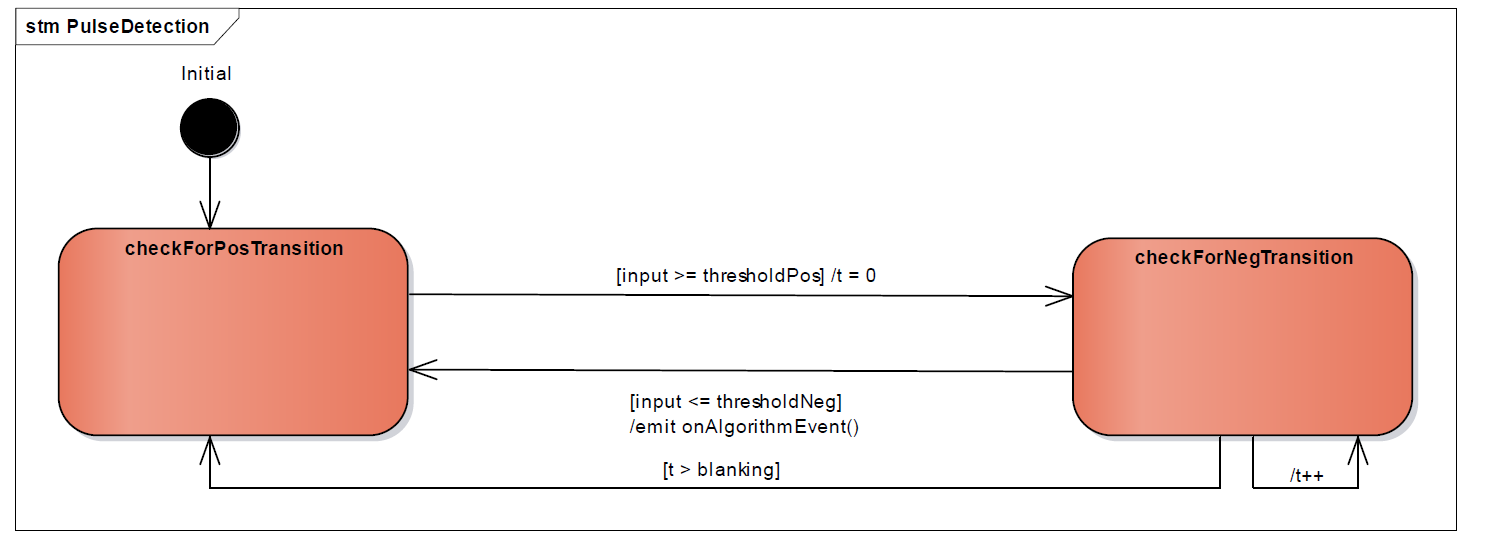
\includegraphics[width=1\linewidth]{900-Praktika/prak08/3.PNG}
\end{center}

\begin{enumerate}
  \item Implementieren Sie die Finite State Machine.
\item  Testen Sie die korrekte Funktion mit dem Test Case PulseDetectorTest des ECG Unit Tests.
\end{enumerate}

\subsubsection{Lösung}

Die Detektion basiert auf den Samples der Ableitung des EKG-Signals, einer positiven und einer negativen Detektionsschwelle (im Diagramm \textit{input, thresholdPos und thresholdNeg}). Zusätzlich existiert ein zeitli-ches Kriterium, damit sichergestellt ist, dass keine Störungen als Puls detektiert werden: unterschreitet die Ableitung die positive Schwelle, muss innerhalb von \textit{blanking}-Samples auch die negative Schwelle über-schritten werden. Ansonsten handelt es sich mit grosser Wahrscheinlichkeit nicht um einen Herzschlag.

\begin{enumerate}
  \item siehe Klasse PulseDetector in ./Loesung/Ecg/algo/PulseDetector.h
\item  Alle Unit Test Cases muss fehlerfrei ausgeführt werden können. Siehe Eclipse-Projekt in ./Loesung/Ecg
\end{enumerate}

\lstinputlisting[language=C++, style=C++, multicols=2]{900-Praktika/prak08/Loesung/Ecg/algo/Algorithm.h}

\newpage
\section{Lab 9 Code Bloat bei Templates, Code Hoisting}
%!TEX root = ../prak.tex
\section{Lab 9 Code Bloat bei Templates, Code Hoisting}
\subsection{Aufgabe 1: Untersuchung von Assemblercode bei Templates}

Die folgenden Optionen der GNU-Compiler könnten nützlich sein:

‐E \qquad  Precompile only, der Output wird auf stdout geschrieben\\
‐S \qquad Assembleroutput, ohne Objectfile erzeugen\\
‐c \qquad nur compilieren\\
‐O0\quad  keine Optimierung\\
‐O1\quad  Optimierungsstufe 1 (siehe g++ - Help für Details)\\
‐O2\quad  Optimierungsstufe 2\\
‐O3\quad  Optimierungsstufe 3\\
‐Os\quad  Optimierung auf Codegrösse\\

\textbf{Hinweis}
Jede Funktion in einem Objectfile oder Binary liegt an einer bestimmten Adresse und ist mit einem Symbol benannt, sofern im Debugmodus compiliert wurde. Mit dem Befehl nm [‐C] [objfile] kann der Inhalt einer solchen Datei ausgegeben werden. Mit der Option –C werden die Symbolnamen demangled. Siehe dazu auch die entsprechende man page.

\begin{enumerate}
  \item  Untersuchen Sie den Code im Verzeichnis ./Vorgabe/StackTemplate. Verschaffen Sie sich einen Überblick und werden Sie vertraut mit der Templateprogrammierung. Beachten Sie, dass einzelne Elementfunktionen implizit inline sind.
  \item Compilieren Sie den Code mit den Optimierungsstufen 0 und 3. Untersuchen Sie jeweils den entstandenen Assemblercode sowie die Codegrösse. Achten Sie vor allem darauf, ob die Funktionen aufgerufen werden (mit call) oder inline sind. Sind die Funktionen einfach oder mehrfach vorhanden?
  \item Ändern Sie den Code nun so ab, dass im Hauptprogramm ein zweiter int-Stack mit unterschiedlicher Grösse definiert wird. Compilieren Sie den Code wiederum unter Verwendung der Optimierungsstufen 0 und 3. Untersuchen Sie jeweils den entstandenen Assemblercode sowie die Codegrösse. Achten Sie darauf, ob die Funktionen aufgerufen werden (mit call) oder inline sind. Sind die Funktionen einfach oder mehrfach vorhanden?
\end{enumerate}

\subsubsection{Lösung}
Alle Programme wurden mit dem Compiler g++ v7.4.0 übersetzt.
\begin{enumerate}
  \item just do it.
  \item  Wenn mit Optimierungsstufe 0 compiliert wird, sind keine Elementfunktionen inline. Alle Elementfunktionen sind einfach vorhanden und werden mit call aufgerufen. Bei Optimierungstufe 3 sind sämtliche Funktionen der Klasse Stack inline. In der folgenden Tabelle sind die Codegrössen ersichtlich.
\begin{center}
  \begin{tabular}{c c c c c}
    \hline
    \hline
    Optimierung O… & g++ v4.7.3 Cygwin & g++ v4.8.4  & g++ v5.4.0 & g++ v7.4.0 \\
    \hline
    0 &
    61'738&
    13‘913&
    14‘024&
    13‘712\\
    3&
    60'043&
    13‘369&
    13‘480&
    13‘120\\
    \hline
    \hline
  \end{tabular}
\end{center}

  \item siehe ./Loesung/A1

\lstinputlisting[language=C++, style=C++, multicols=2]{900-Praktika/prak09/Loesung/A1/Stack.h}
\noindent\makebox[\linewidth]{\rule{\paperwidth}{0.4pt}}
\lstinputlisting[language=C++, style=C++, multicols=2]{900-Praktika/prak09/Loesung/A1/Stack.cpp}
\noindent\makebox[\linewidth]{\rule{\paperwidth}{0.4pt}}
\lstinputlisting[language=C++, style=C++, multicols=2]{900-Praktika/prak09/Loesung/A1/StackUI.h}
\noindent\makebox[\linewidth]{\rule{\paperwidth}{0.4pt}}
\lstinputlisting[language=C++, style=C++, multicols=2]{900-Praktika/prak09/Loesung/A1/StackUI.cpp}
\noindent\makebox[\linewidth]{\rule{\paperwidth}{0.4pt}}
\lstinputlisting[language=C++, style=C++, multicols=2]{900-Praktika/prak09/Loesung/A1/StackTest.cpp}

  Wenn ohne Optimierung compiliert wird, sind keine Elementfunktionen inline. Alle Elementfunktionen inklusive die Konstruktoren sind doppelt mit praktisch identischem Code vorhanden und werden mit call aufgerufen. Die Texte, die mit cout ausgegeben werden, sind nur einfach vorhanden.

\begin{lstlisting}[language=C++, style=C++, multicols=2]
Build mit -O0:
$ nm -C StackTest
...
0000000000000f90 W Stack<int, 3>::pop()
0000000000000f1e W Stack<int, 3>::push(int const&)
0000000000000ab2 W Stack<int, 3>::Stack()
0000000000000ab2 W Stack<int, 3>::Stack()
00000000000010c2 W Stack<int, 4>::pop()
0000000000001050 W Stack<int, 4>::push(int const&)
0000000000000ce8 W Stack<int, 4>::Stack()
0000000000000ce8 W Stack<int, 4>::Stack()
0000000000000ad0 W StackUI<int, 3>::dialog()
0000000000000a7a W StackUI<int, 3>::StackUI()
0000000000000a7a W StackUI<int, 3>::StackUI()
0000000000000d06 W StackUI<int, 4>::dialog()
0000000000000a96 W StackUI<int, 4>::StackUI()
0000000000000a96 W StackUI<int, 4>::StackUI()
0000000000000fec W Stack<int, 3>::peek() const
0000000000001182 W Stack<int, 3>::isFull() const
000000000000103a W Stack<int, 3>::isEmpty() const
0000000000000f7e W Stack<int, 3>::wasError() const
000000000000111e W Stack<int, 4>::peek() const
000000000000119a W Stack<int, 4>::isFull() const
000000000000116c W Stack<int, 4>::isEmpty() const
00000000000010b0 W Stack<int, 4>::wasError() const
...


Build mit -O3:
$ nm -C StackTest
...
0000000000000a80 W StackUI<int, 3>::dialog()
0000000000000d50 W StackUI<int, 4>::dialog()
...
\end{lstlisting}
  Bei älteren Compilerversionen (z.B. g++-Version v3.4.4) waren mit Optimierungstufe 3 nur die impliziten inline-Elementfunktionen inline. Alle weiteren Elementfunktionen waren ebenfalls doppelt vorhanden und wurden mit call aufgerufen. Wenn hingegen g++ v4.8.4, g++ v5.4.0 oder g++ v7.4.0 genommen wird, sind alle Elementfunktionen ausser \texttt{StackUI::dialog()} inline. Diese Funktion ist dann zweifach vorhanden, je für einen Stack der Grösse 3 und der Grösse 4, und wird wie folgt aufgerufen:

\begin{lstlisting}[language=C++, style=C++]
call _ZN7StackUIIiLi3EE6dialogEv
...
call _ZN7StackUIIiLi4EE6dialogEv
\end{lstlisting}
In der folgenden Tabelle sind die Codegrössen ersichtlich.
\begin{center}
  \begin{tabular}{c c c c c}
    \hline
    \hline
    Optimierung O… & g++ v4.7.3 Cygwin & g++ v4.8.4  & g++ v5.4.0 & g++ v7.4.0 \\
    \hline
    0 &
66'052&
14‘440&
14‘544&
14‘240\\
3&
61'389&
13‘420&
13‘528&
13‘168\\
    \hline
    \hline
  \end{tabular}
\end{center}
\end{enumerate}

\subsection{Aufgabe 2: Verhindern von Code Bloat durch Code Hoisting}
In dieser Aufgabe soll untersucht werden, wie mittels Code Hoisting der bei Templates häufig entstehende Code Bloat vermieden werden kann. Die heutigen Compiler erzeugen zwar immer besseren Code. Es ist trotzdem sinnvoll, mittels Code Hoisting möglichen Code Bloat zu vermeiden.

Die Klasse \texttt{StackUI} lassen wir unverändert. Analysieren Sie, welche Teile in der Klasse \texttt{Stack} unabhängig von der Grösse sind. Lagern Sie alle diese Teile in eine Basisklasse aus. Compilieren Sie den Code wiederum mit den Optimierungsstufen 0 und 3. Untersuchen Sie jeweils den entstandenen Assemblercode. Achten Sie darauf, ob die Funktionen aufgerufen werden (mit \texttt{call}) oder inline sind. Sind die Funktionen einfach oder mehrfach vorhanden?

\subsubsection{Lösung}
Code hoisting, siehe ./Loesung/A2. Beachten Sie auch die Kommentare im Source Code.

In der Klasse Stack sollen alle von der Grösse unabhängigen Teile in eine Basisklasse ausgelagert werden. Die Analyse, was unabhängig von der Grösse ist, ist nicht so trivial. Sind beispielsweise die Elementfunktionen isEmpty() und isFull() unabhängig von der Grösse oder nicht? Weiss man das bereits bei der Deklaration oder ist es erst bei der Implementation bekannt? Aus der Implementation geht hervor, dass die Methode isEmpty() unabhängig ist, isFull() jedoch nicht. Alle weiteren Elementfunktionen, die isFull() benötigen, sind demnach auch nicht unabhängig, das ist z.B. push().

Damit die Unterklassen einfach auf die Attribute zugreifen können, sollten top und error als protected statt private definiert werden. In der Basisklasse ist der Array elems[] nicht bekannt, da dieser ja eben abhängig von der Grösse ist. Also müssten beinahe alle Elementfunktionen (alle, die auf den Array zugreifen) in die Unterklasse. Um das zu verhindern, kann im Ctor der Basisklasse ein Pointer auf den elems-Array gesetzt werden. In der Basisklasse wird dann damit gearbeitet. Dies ist zwar nicht gerade schön, allerdings löst es den Code Bloat. Man beachte, dass der Ctor von StackNoSize protected gesetzt wird, damit nur eine Unterklasse diesen aufrufen kann.

Wenn ohne Optimierung compiliert wird, sind keine Elementfunktionen inline. Alle Elementfunktionen und Konstruktoren der Basisklasse sind nur noch einfach vorhanden, alle anderen Elementfunktionen sind doppelt vorhanden
.
Bei älteren Compilerversionen (z.B. g++-Version v3.4.4) waren mit Optimierungstufe 3 die impliziten inline-Elementfunktionen inline. Funktionen der Basisklasse waren nur noch einfach, alle anderen Funktionen doppelt vorhanden. Wenn hingegen g++ v7.4.0 genommen wird, sind alle Elementfunktionen ausser StackUI::dialog() inline. Diese Funktion ist dann zweifach vorhanden, je für einen Stack der Grösse 3 und der Grösse 4.

\lstinputlisting[language=C++, style=C++, multicols=2]{900-Praktika/prak09/Loesung/A2/Stack.h}
\noindent\makebox[\linewidth]{\rule{\paperwidth}{0.4pt}}
\lstinputlisting[language=C++, style=C++, multicols=2]{900-Praktika/prak09/Loesung/A2/Stack.cpp}
\noindent\makebox[\linewidth]{\rule{\paperwidth}{0.4pt}}
\lstinputlisting[language=C++, style=C++, multicols=2]{900-Praktika/prak09/Loesung/A2/StackNoSize.h}
\noindent\makebox[\linewidth]{\rule{\paperwidth}{0.4pt}}
\lstinputlisting[language=C++, style=C++, multicols=2]{900-Praktika/prak09/Loesung/A2/StackNoSize.cpp}
\noindent\makebox[\linewidth]{\rule{\paperwidth}{0.4pt}}
\lstinputlisting[language=C++, style=C++, multicols=2]{900-Praktika/prak09/Loesung/A2/StackUI.h}
\noindent\makebox[\linewidth]{\rule{\paperwidth}{0.4pt}}
\lstinputlisting[language=C++, style=C++, multicols=2]{900-Praktika/prak09/Loesung/A2/StackUI.cpp}
\noindent\makebox[\linewidth]{\rule{\paperwidth}{0.4pt}}
\lstinputlisting[language=C++, style=C++, multicols=2]{900-Praktika/prak09/Loesung/A2/StackTest.cpp}

\begin{center}
  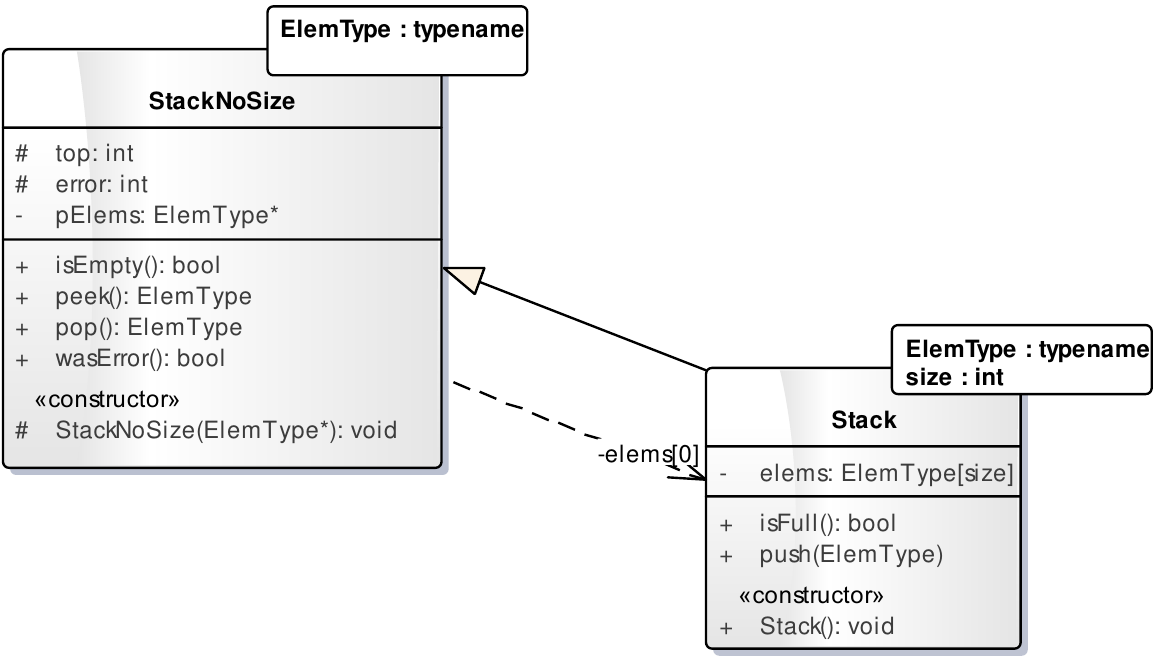
\includegraphics[width=.6\linewidth]{900-Praktika/prak09/1.PNG}
\end{center}

\newpage
\section{Lab 10 Dynamic Memory Management}
%!TEX root = ../prak.tex
\section{Lab 10 Dynamic Memory Management}
\subsection{Aufgabe 1: Fixed-size Pool}
Ihre Aufgabe ist es, einen Fixed-size Pool in Anlehnung an die in der Vorlesung gezeigte Variante zu implementieren. Sie müssen die Klassen \texttt{PoolAllocator, HeapException, HeapSizeMismatch und OutOfHeap} realisieren, wobei die letzten beiden Klassen Unterklassen von HeapException sind. Die Exceptionklassen müssen möglichst schlank implementiert werden (was heisst das?).
Packen Sie alle Klassendeklarationen in das File \texttt{PoolAllocator.h}, definieren Sie sehr kurze Elementfunktionen implizit \texttt{inline}, alle weiteren separat, ebenfalls im File \texttt{PoolAllocator.h}. Alle Klassen müssen in den Namespace \texttt{dynamicMemory} gelegt werden. Nachfolgend finden Sie einen Ausschnitt aus der Deklaration der Klasse \texttt{dynamicMemory::PoolAllocator}.

\begin{lstlisting}[language=C++, style=C++]
template<std::size_t heapSize, std::size_t elemSize>
class PoolAllocator
{
  public:
    PoolAllocator(/* TODO: params (heap address */);
    void* allocate(std::size_t bytes);
    // TODO: implement this
    // throw a HeapSizeMismatch Exception if 'bytes' doesn't match elemSize
    // throw a OutOfHeap Exception if requested 'bytes' aren't available
    void deallocate(/* TODO: params */) noexcept;
    // TODO: implement this
    // add this element to the freelist
    // set the pointer to nullptr
  private:
    union Node
    {
        uint8_t data[elemSize]; // sizeof(data) should be >= sizeof(Node*)
        Node* next;
    };
    Node* freeList;
  };
  template<std::size_t heapSize, std::size_t elemSize>
  PoolAllocator<heapSize, elemSize>::PoolAllocator(uint8_t* heapAddr)
  {
  // TODO: implement this
}
\end{lstlisting}

Das Testprogramm finden Sie im Verzeichnis ./Vorgabe. Der Output des Testprogramms soll wie folgt aussehen (Die Anfangsadresse kann unterschiedlich sein):

\begin{lstlisting}[language=C++, style=C++]
p[0] = 0x7ffe93438070
p[1] = 0x7ffe93438078
p[2] = 0x7ffe93438080
p[1] = 0
p[3] = 0x7ffe93438078
Heapsize mismatch exception occurred
\end{lstlisting}

\begin{enumerate}
  \item Implementieren und testen Sie die Klassen vollständig. Erweitern Sie das Testprogramm so, dass auch eine OutOfHeap-Exception geprüft wird.
\item Erweitern Sie die Elementfunktion \texttt{dynamicMemory::PoolAllocator::allocate()} so, dass die Anzahl der angeforderten Bytes nicht mehr genau der Elementgrösse entsprechen muss, sondern kleiner oder gleich der Elementgrösse sein kann.
\end{enumerate}

\subsubsection{Lösung}

\begin{enumerate}
  \item Beachten Sie den Referenzparameter in \texttt{void deallocate(void*\& ptr) throw()}. Dadurch ist es ohne Doppelpointer möglich, \texttt{ptr} auf \texttt{nullptr} zu setzen.

  \lstinputlisting[language=C++, style=C++, multicols=2]{900-Praktika/prak10/Loesung/FixedPool/src/PoolAllocator.h}
  \noindent\makebox[\linewidth]{\rule{\paperwidth}{0.4pt}}
  \lstinputlisting[language=C++, style=C++, multicols=2]{900-Praktika/prak10/Loesung/FixedPool/src/FixedPool.cpp}

  \item Die einzige Änderung muss in der Elementfunktion \texttt{void* allocate()} vorgenommen werden. Der Operator != muss durch den $>$-Operator ersetzt werden:
\begin{lstlisting}[language=C++, style=C++]
if (bytes > elemSize) // objects smaller than elemSize are allowed
  throw HeapSizeMismatch();
\end{lstlisting}
\lstinputlisting[language=C++, style=C++, multicols=2]{900-Praktika/prak10/Loesung/FixedPoolCeil/src/PoolAllocator.h}
\noindent\makebox[\linewidth]{\rule{\paperwidth}{0.4pt}}
\lstinputlisting[language=C++, style=C++, multicols=2]{900-Praktika/prak10/Loesung/FixedPoolCeil/src/FixedPoolCeil.cpp}
\end{enumerate}


\subsection{Aufgabe 2: Block Allocator}
Implementieren Sie nun einen Block Allocator. Die Klasse \texttt{BlockAllocator} soll aus 4 Fixed-size Pools gemäss Aufgabe 1b) bestehen. Die einzelnen Elementgrössen können der Klasse \texttt{BlockAllocator} mittels Templateparameter mitgegeben werden. Der Block Allocator nimmt jeweils den kleinstmöglichen Pool, um die Anforderungen zu erfüllen. Das bedeutet auch, dass auf den nächstgrösseren Pool zugegriffen wird, falls der kleinere Pool voll ist.
\lstinputlisting[language=C++, style=C++, multicols=2]{900-Praktika/prak10/Loesung/BlockAllocation/src/PoolAllocator.h}
\noindent\makebox[\linewidth]{\rule{\paperwidth}{0.4pt}}
\lstinputlisting[language=C++, style=C++, multicols=2]{900-Praktika/prak10/Loesung/BlockAllocation/src/BlockAllocator.h}
\noindent\makebox[\linewidth]{\rule{\paperwidth}{0.4pt}}
\lstinputlisting[language=C++, style=C++, multicols=2]{900-Praktika/prak10/Loesung/BlockAllocation/src/BlockAllocation.cpp}

\newpage
\section{Lab 11 C++ and ROMability, Hardware Abstraction Layer (HAL)}
\subsection{Aufgabe 1: C++ and ROMability, Hardware Abstraction Layer (HAL)}

In der Vorlesung haben wir gesehen, dass unterschiedliche Konstrukte ROMable sind, jedoch nicht jeder
Compiler diese Konstrukte auch im ROM platziert. In dieser Aufgabe untersuchen Sie die ROMability und die
Optimierung von ROMable Konstrukten des g++-Compilers. Für die Untersuchung müssen Sie unter Umständen
Optimierungsstufen setzen.

Die folgenden Optionen des GNU-Compilers können für diese Aufgabe nützlich sein:

\medskip
\noindent<
‐E  \qquad Precompile only, der Output wird auf stdout geschrieben\\
‐S  \qquad Assembleroutput, ohne Objectfile erzeugen\\
‐c \qquad nur compilieren\\
‐O0 \qquad keine Optimierung\\
‐O1 \qquad Optimierungsstufe 1 (siehe g++ ‐‐help oder man g++ für Details)\\
‐O2 \qquad Optimierungsstufe 2\\
‐O3 \qquad Optimierungsstufe 3\\
‐Os \qquad Optimierung auf Codegrösse\\

\textbf{Achten Sie bei allen Untersuchungen darauf, dass Ihre kleinen Testprogramme nicht vollständig
wegoptimiert werden, da die definierten Variablen nicht weiterverwendet werden. Damit das nicht
passiert, können Sie den Inhalt der Variablen in die Console schreiben.}

\begin{enumerate}
  \item  Umsetzung von Strings: Untersuchen Sie, wie die untenstehenden Stringdefinitionen umgesetzt werden.
Wird \textit{World} mit \textit{Hello World} gemeinsam verwendet? Gibt es allenfalls Unterschiede in Abhängigkeit
der Optimierungsstufen?

\texttt{
const char* pc1 = "Hello World";\\
const char* const pc2 = "World";}

\item Wie werden Tabellen umgesetzt? Gibt es einen Unterschied in der Umsetzung der folgenden beiden Definitionen?
Was passiert, wenn Sie beiden Definitionen das Schlüsselwort static voranstellen?

\texttt{const int table1[] = {1, 2, 3};\\
int table2[] = {1, 2, 3};}

\item Integerkonstanten: Für die Definition von Integerkonstanten stehen Ihnen drei Möglichkeiten zur Verfügung:
const int, enum und \#define. Wie werden diese Varianten umgesetzt? Geben Sie in Ihrem
Testprogramm dem Compiler die Chance, eine Immediate-Adressierung zu verwenden. Um herauszufinden,
ob eine Konstante mehrfach im Speicher angelegt wird (ohne Immediate-Adressierung), müssen
Sie die definierte Konstante mehrfach im Programm verwenden.
\item Floating Point-Konstanten: Für die Definition von Floating Point-Konstanten stehen Ihnen const double
und \#define zur Verfügung. Wie werden diese Varianten umgesetzt? Eine Immediate-Adressierung ist
mit doubles kaum möglich. Um herauszufinden, ob eine Konstante mehrfach im Speicher angelegt wird,
müssen Sie die definierte Konstante mehrfach im Programm verwenden.
\item Können Sie herausfinden, ob vtbl's im ROM abgelegt werden?
\end{enumerate}

\subsubsection{Lösung}

\begin{enumerate}
  \item  siehe ./Loesung/A1-0
Solange die Strings völlig identisch sind (Formatstring), wird der String nur einmal im Speicher abgelegt. Bei Teilstrings werden bei jeder Optimierungsstufe beide Strings vollständig gespeichert (doppelt). Wenn nur der String ausgegeben wird, ersetzt der Compiler printf() durch puts(). Bei dieser speziellen An-wendung spart man sich dadurch den Formatstring (hier ist g++ smart).
\lstinputlisting[language=C++, style=C++, multicols=2]{900-Praktika/prak11/Loesung/A1-0/main.cpp}
\noindent\makebox[\linewidth]{\rule{\paperwidth}{0.4pt}}
\lstinputlisting[language=C++, style=C++, multicols=2]{900-Praktika/prak11/Loesung/A1-0/main.s}
\noindent\makebox[\linewidth]{\rule{\paperwidth}{0.4pt}}
  \item siehe ./Loesung/A1-1
Solange von beiden Tabellen nur gelesen wird, könnten beide Tabellen geROMt werden, bzw. sogar nur einfach gespeichert werden, da der Inhalt identisch ist.
Diese kurzen Tabellen werden sogar auf dem Stack abgespeichert. Sobald sie grösser sind, werden sie ebenfalls im Datenbereich gespeichert.
Interessant sind vor allem noch die folgenden Deklarationen mit static. static bewirkt, dass die Ta-bellen auf jeden Fall im Datenbereich gespeichert werden, d.h. keinesfalls mehr auf dem Stack. const bewirkt, dass die Tabellen in den read-only Bereich gehen.

\texttt{static const int table1[] = {1, 2, 3}; static int table2[] = {1, 2, 3};}


\lstinputlisting[language=C++, style=C++, multicols=2]{900-Praktika/prak11/Loesung/A1-1/main.cpp}
\noindent\makebox[\linewidth]{\rule{\paperwidth}{0.4pt}}
\lstinputlisting[language=C++, style=C++, multicols=2]{900-Praktika/prak11/Loesung/A1-1/main.s}
\noindent\makebox[\linewidth]{\rule{\paperwidth}{0.4pt}}

  \item siehe ./Loesung/A1-2
Integerkonstanten, die mit \#define oder enum definiert sind, jedoch nicht gebraucht werden, ergeben weder Code noch Daten. Integerkonstanten, die mit const definiert sind, werden auch dann gespeichert, wenn sie gar nicht verwendet werden, damit die Konstanten vorhanden sind, falls eine andere Compilationseinheit diese Konstanten verwenden würde. Innerhalb des .cpp-Files der Konstantendefinition wer-den diese Konstanten ebenfalls mittels Immediate-Adressierung verwendet.
Die beste Variante, um Integerkonstanten zu definieren, ist eindeutig mittels enum. \#defines haben die bekannten Makroprobleme, consts brauchen unnötigerweise Speicher.

\lstinputlisting[language=C++, style=C++, multicols=2]{900-Praktika/prak11/Loesung/A1-2/main.cpp}
\noindent\makebox[\linewidth]{\rule{\paperwidth}{0.4pt}}
\lstinputlisting[language=C++, style=C++, multicols=2]{900-Praktika/prak11/Loesung/A1-2/main.s}
\noindent\makebox[\linewidth]{\rule{\paperwidth}{0.4pt}}
\lstinputlisting[language=C++, style=C++, multicols=2]{900-Praktika/prak11/Loesung/A1-2/ints.h}
\noindent\makebox[\linewidth]{\rule{\paperwidth}{0.4pt}}
\lstinputlisting[language=C++, style=C++, multicols=2]{900-Praktika/prak11/Loesung/A1-2/subs.cpp}
\noindent\makebox[\linewidth]{\rule{\paperwidth}{0.4pt}}
\lstinputlisting[language=C++, style=C++, multicols=2]{900-Praktika/prak11/Loesung/A1-2/subs.s}
\noindent\makebox[\linewidth]{\rule{\paperwidth}{0.4pt}}
  \item siehe ./Loesung/A1-3
Gleitpunktkonstanten können normalerweise (speziell bei Mikrocontrollern) nicht mittels Immediate-Ad-ressierung verwendet werden, d.h. es ist immer eine Konstante im Datenbereich vorhanden. Bei 64 Bit-Systemen (z.B. unsere Laborrechner) kann ein Register einen ganzen double-Wert (8 Byte) beinhalten, die Instruktion MOVABSQ (Move quad word to register) lädt einen double-Wert mittels Immediateadressie-rung direkt in ein solches Register. Konstanten, die mit \#define definiert sind, jedoch nicht gebraucht werden, ergeben weder Code noch Daten. Gleitpunktkonstanten, die mit const definiert sind, werden auch dann gespeichert, wenn sie gar nicht verwendet werden, damit die Konstanten vorhanden sind, falls eine andere Compilationseinheit diese Konstanten verwenden würde. Allerdings sind diese Konstanten immer nur einfach vorhanden. Konstanten, die mit \#define definiert wurden, sind in jeder Compilationseinheit separat, d.h. mehrfach vorhanden.Die beste Variante, um Gleitpunktkonstanten zu definieren, ist nicht so eindeutig festzulegen. \#defines haben die bekannten Makroprobleme und benötigen allenfalls mehrfach Speicher für densel-ben Wert, jedoch nur, wenn sie wirklich verwendet werden. consts brauchen leider auch Speicher, wenn sie gar nicht verwendet werden, allerdings nur einmal. Solange nicht zu viele consts auf Vorrat definiert werden, schlage ich vor, auch hier auf \#defines zu verzichten und consts zu verwenden. Gute Compiler/ Linker mit Link-Time Optimization (LTO) sollten nicht verwendete Konstanten entfernen.
  \item siehe ./Loesung/A1-4
  \lstinputlisting[language=C++, style=C++, multicols=2]{900-Praktika/prak11/Loesung/A1-3/main.cpp}
  \noindent\makebox[\linewidth]{\rule{\paperwidth}{0.4pt}}
  \lstinputlisting[language=C++, style=C++, multicols=2]{900-Praktika/prak11/Loesung/A1-3/main.s}
  \noindent\makebox[\linewidth]{\rule{\paperwidth}{0.4pt}}
  \lstinputlisting[language=C++, style=C++, multicols=2]{900-Praktika/prak11/Loesung/A1-3/floats.h}
  \noindent\makebox[\linewidth]{\rule{\paperwidth}{0.4pt}}
  \lstinputlisting[language=C++, style=C++, multicols=2]{900-Praktika/prak11/Loesung/A1-3/subs.cpp}
  \noindent\makebox[\linewidth]{\rule{\paperwidth}{0.4pt}}
  \lstinputlisting[language=C++, style=C++, multicols=2]{900-Praktika/prak11/Loesung/A1-3/subs.s}
  \noindent\makebox[\linewidth]{\rule{\paperwidth}{0.4pt}}
\end{enumerate}

Die vtbl's werden in den Abschnitt rodata, d.h. read-only data gelegt (\_ZTV1A und \_ZTV1B). Bei einem Embedded System mit ROM könnte dieser Bereich ins ROM gelegt werden.

\subsection{Aufgabe 2: Ohne Hardware Abstraction Layer}

Im Vorgabeordner finden Sie eine Beispielapplikation für den EswRobot. Die Applikation initialisiert den Roboter
und lässt LED 1 leuchten solange Switch 1 gedrückt wird und lässt LED 2 leuchten solange Switch 2
gedrückt wird. Die komplette Funktionalität wurde im File main.c implementiert, ohne eine HAL zu verwenden.

Die folgenden Aufgaben sollen aufzeigen wie eine HAL eingesetzt und implementiert werden kann. Durch
den HAL soll der Code leserlich und erweiterbar gestaltet werden können, ohne dabei auf Performance verzichten
zu müssen. Die Implementation ohne HAL stellt die Baseline für die Implementation mit HAL dar.

\begin{enumerate}
  \item Importieren Sie das Projekte NoHAL (./Vorgabe/NoHAL) ins Code Composer Studio und studieren Sie
den Code im File main.c.
\item Definieren Sie die fehlenden GIO A Registeradressen. Informationen über die Register finden Sie im
"Technical Reference Manual". Das Memory Map und die Registeradressen finden Sie im Datenblatt des
TMS320F2806x Microcontrollers. In "Table 6-70. GPIO Registers" sind die Registeradressen für die GIO
Peripherie aufgelistet.
\item Verifizieren Sie die Funktionalität der Applik
\end{enumerate}

\subsubsection{Lösung}

\begin{enumerate}
  \item just do it
  \item \lstinputlisting[language=C++, style=C++, multicols=2]{900-Praktika/prak11/Loesung/NoHAL/main.c}
\end{enumerate}

\subsection{Aufgabe 3: Hardware Abstraction Layer in C}

Um die Applikation leserlich und erweiterbar zu gestalten, wird der Microcontroller in einer Chip Support Library
(CSL) und das PCB des EswRobot in einer Board Support Library (BSL) abstrahiert. Diese beiden Libraries
bilden den Hardware Abstraction Layer (HAL). Diese Abstraktion wurde für den EswRobot im Projekt
CHAL in C vorgenommen.

\begin{enumerate}
  \item Importieren Sie das Projekte CHAL (./Vorgabe/CHAL) ins Code Composer Studio und studieren Sie die
CSL und die BSL.
\item  Implementieren Sie die gleiche Funktionalität wie im Projekt NoHAL mit Hilfe des vorgegebenen HALs in
main.c.
\item Verifizieren Sie, ob Ihr Testprogramm einwandfrei funktioniert.
\end{enumerate}

\subsubsection{Lösung}
\begin{enumerate}
  \item just do it
  \item \lstinputlisting[language=C++, style=C++, multicols=2]{900-Praktika/prak11/Loesung/CHAL/main.c}
  \item \lstinputlisting[language=C++, style=C++, multicols=2]{900-Praktika/prak11/Loesung/CHAL/bsl/include/led.h}
  \noindent\makebox[\linewidth]{\rule{\paperwidth}{0.4pt}}
  \lstinputlisting[language=C++, style=C++, multicols=2]{900-Praktika/prak11/Loesung/CHAL/bsl/include/switch.h}
  \noindent\makebox[\linewidth]{\rule{\paperwidth}{0.4pt}}
  \lstinputlisting[language=C++, style=C++]{900-Praktika/prak11/Loesung/CHAL/csl/include/bits.h}
  \noindent\makebox[\linewidth]{\rule{\paperwidth}{0.4pt}}
  \lstinputlisting[language=C++, style=C++, multicols=2]{900-Praktika/prak11/Loesung/CHAL/csl/include/hwreg.h}
  \noindent\makebox[\linewidth]{\rule{\paperwidth}{0.4pt}}
  \noindent\makebox[\linewidth]{\rule{\paperwidth}{0.4pt}}
  \lstinputlisting[language=C++, style=C++, multicols=2]{900-Praktika/prak11/Loesung/CHAL/csl/include/pin.h}
  \lstinputlisting[language=C++, style=C++, multicols=2]{900-Praktika/prak11/Loesung/CHAL/csl/include/port.h}
  \noindent\makebox[\linewidth]{\rule{\paperwidth}{0.4pt}}
  \lstinputlisting[language=C++, style=C++, multicols=2]{900-Praktika/prak11/Loesung/CHAL/csl/src/pin.c}
  \noindent\makebox[\linewidth]{\rule{\paperwidth}{0.4pt}}
  \lstinputlisting[language=C++, style=C++, multicols=2]{900-Praktika/prak11/Loesung/CHAL/csl/src/port.c}
  \noindent\makebox[\linewidth]{\rule{\paperwidth}{0.4pt}}
  \lstinputlisting[language=C++, style=C++, multicols=2]{900-Praktika/prak11/Loesung/CHAL/csl/src/protHwRegAccess.h}
  \noindent\makebox[\linewidth]{\rule{\paperwidth}{0.4pt}}

\end{enumerate}

\subsection{Aufgabe 4: Hardware Abstraction Layer in C++}
Im Projekt CHAL wurde die Applikation vom Projekt NoHAL mit einem HAL in C implementiert. In dieser Aufgabe
wird dieselbe Funktionalität mit einem HAL in C++ implementiert.

\begin{enumerate}
  \item  Importieren Sie das Projekte CPPHAL (./Vorgabe/CPPHAL) ins Code Composer Studio und studieren Sie
die CSL, die BSL und die main()-Funktion.
\item  Die Schnittstelle für die BSL Klassen Led und Switch sind definiert, aber nicht implementiert. Implementieren
Sie die beiden Klassen vollständig. Alle Funktionen müssen implizit inline implementiert werden.
\item Verifizieren Sie, ob das vorgegebene Testprogramm einwandfrei funktioniert.
\end{enumerate}

\subsubsection{Lösung}


\begin{enumerate}
  \item just do it
  \item \lstinputlisting[language=C++, style=C++, multicols=2]{900-Praktika/prak11/Loesung/CPPHAL/bsl/include/Led.h}
  \noindent\makebox[\linewidth]{\rule{\paperwidth}{0.4pt}}
  \lstinputlisting[language=C++, style=C++, multicols=2]{900-Praktika/prak11/Loesung/CPPHAL/bsl/include/Switch.h}
  \noindent\makebox[\linewidth]{\rule{\paperwidth}{0.4pt}}
\end{enumerate}

\subsection{Aufgabe 5: Hardware Abstraction Layer in C++ mit Memory-mapped IO (MMIO)}

Bei Microcontrollern werden die peripheren Module direkt in den Speicher eingebunden und können über
Adressen angesteuert werden. Die Klassen Pin und Port aus der CSL abstrahieren die GPIO-Module des
Microcontrollers und verwenden für die Registerzugriffe Instanzen der Klasse HwReg, welche direkt an die
entsprechende Registeradresse platziert werden.

\begin{enumerate}
  \item  Importieren Sie das Projekte CPPHAL\_advanced (./Vorgabe/CPPHAL\_advanced) ins Code Composer
Studio und studieren Sie die CSL, die BSL und die main()-Funktion.
\item Implementieren Sie die Klasse HwReg vollständig. Alle Funktionen müssen implizit inline implementiert
werden.
\item  Platzieren Sie die benötigten HwReg-Objekte in der Pin Klasse an der korrekten Stelle und implementieren
Sie damit die Stubs. Verwenden Sie die bereits implementierte toggle Methode als Inspiration.
Überlegen Sie sich, ob für die Platzierung placement new oder ein reinterpret\_cast bevorzugt wird?
Hinweis: Für placement new müssen Sie den Header $<$new$>$ inkludieren.
\item Verifizieren Sie, ob das vorgegebene Testprogramm einwandfrei funktioniert.
\item  Compilieren Sie ihren Code mit der Optimierungsstufe O3 und beantworten Sie die folgenden Fragen.
Um die Optimierungsstufe festzulegen, müssen Sie in den Projekteinstellungen unter Build $->$ C2000
Compiler $->$ Optimization das Optimization level 3-Interprocedure Optimization in der Dropdownliste
auswählen.
\begin{enumerate}
  \item  Wie wird die Abfrage if(statusSwitch.pressed()) im main auf Zeile 22 umgesetzt?
  \item  Wie wird die Anweisung statusIndicator.off(); im main auf Zeile 25 umgesetzt?

\end{enumerate}
\end{enumerate}

\subsubsection{Lösung}

\begin{enumerate}
  \item  just do it
\item  siehe ./Loesung/CPPHAL\_advanced/csl/include/HwReg.h
\lstinputlisting[language=C++, style=C++, multicols=2]{900-Praktika/prak11/Loesung/CPPHAL_advanced/csl/include/HwReg.h}


\item In diesem Fall macht ein reinterpret\_cast$<$ HwRegister<uint32\_t$>$*$>$ mehr Sinn, da keine Konstruktoraufruf erwünscht ist. Zudem wird Placement new nicht auf null Instruktionen reduziert. Es wird ein Call und ein Return durchgeführt, obwohl der Placement new Operator nur die übergebene Adresse zurückgibt. Immerhin wird der Konstruktoraufruf auf null Instruktionen reduziert.
Siehe ./Loesung/CPPHAL\_advanced/csl/include/Pin.h
\lstinputlisting[language=C++, style=C++, multicols=2]{900-Praktika/prak11/Loesung/CPPHAL_advanced/csl/include/Pin.h}
\item Bei der Umsetzung mit Optimierungsstufe O3 wurden alle Funktionen von Pin inline, d.h. es wird direkt mit Bitmasken auf den Registern operiert, ohne Overhead zu verursachen.
\begin{enumerate}
  \item Die Adresse des Registers GPADAT wird ins Register XAR4 geladen. Bit 10 im High Byte (Bit 26) wird überprüft und je nach Testergebnis wird gesprungen. Ab Zeile 1354 in Debug/main.asm.
  \begin{lstlisting}[language=C++, style=C++]
  ...
  MOVL       XAR4,#28608      ; [CPU_ARAU] |60|
  TBIT       *+XAR4[1],#10    ; [CPU_ALU] |60|
  B          $C$L24,TC        ; [CPU_ALU] |60|
  ...
  \end{lstlisting}
  \item Die Adresse des Registers GPACLEAR wird ins Register XAR4 geladen. Der Inhalt des Registers wird dann direkt OR verknüpft mit 0x40 (Bit 6) um den LED 1 Pin auf 0 zu setzen. Ab Zeile 1363 in Debug/main.asm.
  \begin{lstlisting}[language=C++, style=C++]
  ...
  $C$L24:
  MOVL        XAR4,#28612 ; [CPU_ARAU] |38|
  $C$L25:
  OR          *+XAR4[0],#64 ; [CPU_ALU] |38|
  ...
  \end{lstlisting}

\end{enumerate}
\end{enumerate}

\newpage
\section{Lab 12 Zufallszahlengeneratoren}
%!TEX root = ../prak.tex
\section{Lab 12 Zufallszahlengeneratoren}
\subsection{Aufgabe 1: Wahrscheinlichkeitsverteilungen}
Implementieren Sie die Klasse RandIntGen, die Ihnen unterschiedlich verteilte ganze Zahlen liefert. Als User Interface genügt die Console. In der Klasse sollen keinerlei Userinteraktionen (cin, cout, etc.) vorhanden sein. Die Klasse soll die folgenden Methoden anbieten:

\noindent
\texttt{getUniform(); // liefert eine gleichverteilte ganze Zahl\\
getNormal(); // liefert eine normalverteilte ganze Zahl\\
getWeibull(); // liefert eine Weibull‐verteilte ganze Zahl}

\begin{enumerate}
  \item Definieren Sie die Schnittstelle. Überlegen Sie sich dabei, welche Methoden notwendig sind, und wie die Parameter und Returnwerte aussehen müssen, inkl. die korrekte Anwendung von const.
  \item Implementieren Sie Stubs der Klasse.
  \item Implementieren Sie ein Testprogramm, das die Häufigkeit der einzelnen Werte ermittelt und stellen Sie diese Resultate in einem Histogramm (intern oder extern z.B. mit Excel/Matlab/gnuplot) dar.
  \item Führen Sie dieses Programm aus.
  \item Implementieren Sie die Klasse (Methode um Methode).
  \item Verwenden sie die Pseudo-random number generators von C++ und vergleichen Sie die Verteilungen mit den Verteilungen generiert mit der Klasse RandIntGen. Informationen über die Pseudo-random number generators finden sie hier: https://en.cppreference.com/w/cpp/numeric/random
\end{enumerate}

\textbf{Hinweise:}
\begin{itemize}
  \item  Verwenden Sie die in den Vorlesungsunterlagen beschriebenen Formeln.
  \item Die Weibullverteilung besitzt zwei reelle Parameter $\alpha$ und $\beta$. Aus der Gleichverteilung erhält man eine Weibull-verteilte Zahl $w$ wie folgt:
  \begin{enumerate}
    \item Erzeuge eine gleichverteilte Zahl u im Bereich [0, 1[
    \item $w = \beta(-\log(1.0-u)^{\frac{1}{a}})$
  \end{enumerate}
  \item Seien Sie vorsichtig bei der Umrechnung von Gleitpunktwerten in ganzzahlige Werte. Überlegen Sie sich, wann \texttt{lround()} verwendet werden kann und wann \texttt{static\_cast<int>}. Zur Erinnerung: bei der zweiten Methode wird ohne zu runden einfach der ganzzahlige Teil genommen.
  \item Bei gewissen Verteilungen müssen Sie \texttt{lround()} nehmen, bei anderen \texttt{static\_cast<int>}.
\end{itemize}

\subsubsection{Lösung}


\lstinputlisting[language=C++, style=C++, multicols=2]{900-Praktika/prak12/Distributions/src/RandIntGen.h}
\noindent\makebox[\linewidth]{\rule{\paperwidth}{0.4pt}}
\lstinputlisting[language=C++, style=C++, multicols=2]{900-Praktika/prak12/Distributions/src/RandIntGen.cpp}
\noindent\makebox[\linewidth]{\rule{\paperwidth}{0.4pt}}
\lstinputlisting[language=C++, style=C++, multicols=2]{900-Praktika/prak12/Distributions/src/Distributions.cpp}

\newpage
\section{Lab 13 Security}
%!TEX root = ../prak.tex
\section{Lab 13 Security}
\subsection{Aufgabe 1: Hashing}
Im Verzeichnis ./Vorgabe/Hash finden Sie drei JPG-Files, die alle dieselbe Grösse und denselben Timestamp haben. Zwei Dateien sind identisch, eine ist unterschiedlich. Sie sollen herausfinden, welche Datei unterschiedlich ist.
Sie könnten diese Aufgabe mit dem Linux-Befehl diff lösen. Sie könnten die Dateien ebenfalls Byte für Byte binär vergleichen. Sie sollen nun aber diese Aufgabe mit Hilfe einer Hashfunktion lösen. Wenn die Dateien identisch sind, haben Sie denselben Fingerprint.

\subsubsection{Lösung}
Im Windows Explorer kann unter dem Kontextmenu CRC SHA ein Hash Fingerprint einer Datei erstellt werden, z.B. SHA-256. Unter Linux besteht für SHA-256 der Befehl sha256sum. Die SHA-256 Hashes der einzelnen Dateien sind:

img3.jpg: SHA256: EF5CDDD830BBCBF544FFEB18E3B28B4D19D65A5AE16F4618D742683940F9E64D

img4.jpg: SHA256: EF5CDDD830BBCBF544FFEB18E3B28B4D19D65A5AE16F4618D742683940F9E64D

img5.jpg: SHA256: 5E8EDB576C3CF31013ED0858E35C280BA5B667164DA2991C1AE2ECAF90975A2B

Aus den erhaltenen Hashes sieht man, dass die Dateien img3.jpg und img4.jpg identisch sind, img5.jpg aber abweicht. In img5.jpg wurde nur ein einziges Byte abgeändert, die Metainformation "Photoshop" wurde in "Photishop" abgeändert, das eigentliche Bild ist identisch. Man sieht eindrücklich, dass die Änderung eines einzigen Bytes einen völlig anderen Hash ergibt. Das ist unter anderem die Stärke einer guten Hashfunktion.

\subsection{Aufgabe 2: Verschlüsselten Text entschlüsseln}

Eine typische Verschlüsselungsmethode wandelt die Buchstaben eines Textfiles in ASCII und führt Buchstabe um Buchstabe eine XOR-Verknüpfung mit einem Wert aus einem geheimen Schlüssel durch. Die XOR-Funktion ist sehr schnell und sie ist symmetrisch, d.h.

\noindent
\texttt{ciphertextByte = plaintextByte $\oplus$ key und \\
plaintextByte = ciphertextByte $\oplus$ key}


Je länger ein Passwort ist und je mehr unterschiedliche Zeichen es enthält, desto sicherer ist das Passwort. In diesem Beispiel nehmen wir ein Passwort, das nur aus 3 kleinen Buchstaben (a-z) besteht. Der Schlüssel besteht aus der fortlaufenden Aneinanderreihung dieses Passworts.
In ./Vorgabe/Cipher finden Sie einen ciphertext, der mit einem Passwort bestehend aus 3 Kleinbuchstaben verschlüsselt wurde. Ihre Aufgabe besteht darin, das Passwort zu knacken und den Text zu entschlüsseln. Zur Lösung können Sie die folgenden Kenntnisse nutzen:
\begin{itemize}
  \item Das Passwort besteht aus drei Kleinbuchstaben, der Schlüssel wird durch fortlaufendes Aneinanderreihen des Passworts generiert
  \item Die Verschlüsselung geschieht mittels XOR-Funktion
  \item Der unverschlüsselte englische Text besteht nur aus Gross- und Kleinbuchstaben, Ziffern, Leerzeichen und Satzzeichen
\end{itemize}

Als Angriffsvariante können Sie beispielsweise eine oder mehrere der folgenden Strategien anwenden:
\begin{itemize}
  \item Trial and error
  \item Brute force (es gibt 26 * 26 * 26 = 17'576 Möglichkeiten für den Schlüssel)
  \item Intuition, Raten, etc.
  \item Häufigkeitsanalyse der Buchstaben. Die 10 häufigsten Buchstaben der englischen Sprache in abnehmender Reihenfolge sind: e, t, a, o, i, n, s, h, r, d, l.
  \item Erraten einer Teillösung und fortlaufendes Erraten von zusätzlichen Buchstaben
  \item Weitere intelligente Methoden (beachten Sie, dass der Plaintext aus lesbaren Zeichen besteht)
\end{itemize}

\subsubsection{Lösung}
Der folgende Ansatz nutzt die Häufigkeit der verschlüsselten Buchstaben. Bei der verwendeten Verschlüsselungsart (XOR-Verknüpfung) kann aus den Häufigkeiten der verschlüsselten Buchstaben direkt auf die Häufigkeit der unverschlüsselten Buchstaben geschlossen werden.
In der englischen Sprache ist der Buchstabe 'e' der häufigste. Da es sich beim Originaltext um einen Prosatext handelt, ist aber das Leerzeichen (ASCII 0x20) der häufigste Buchstabe.
Der Schlüssel besteht aus drei Kleinbuchstaben. Jeder dritte Originalbuchstabe $x_i, x_{i+3}, x_{i+6}, \ldots$ wurde deshalb mit demselben Schlüsselbuchstaben $k_i$ verschlüsselt, d.h. $y_{i+n\cdot3} = x_{i+n\cdot3} \oplus k_i$. Für den häufigsten (nun bekannten) Buchstaben $y_{i,f}$ gilt:\\
$y_{i,f} = 0x20 \oplus k_i \quad \Rightarrow \quad k_i = 0x20 \oplus y_{i,f}$\\
Dieses Vorgehen muss mit $i = 0, 1, 2$ durchgeführt werden. Damit erhält man direkt den Schlüssel bestehend aus den drei Kleinbuchstaben.

\lstinputlisting[language=C++, style=C++, multicols=2]{900-Praktika/prak13/Loesung/Cipher/CipherFreq/src/CipherFreq.cpp}

\end{document}
